\documentclass[twoside]{book}

% Packages required by doxygen
\usepackage{calc}
\usepackage{doxygen}
\usepackage{graphicx}
\usepackage[utf8]{inputenc}
\usepackage{makeidx}
\usepackage{multicol}
\usepackage{multirow}
\usepackage{textcomp}
\usepackage[table]{xcolor}

% NLS support packages
\usepackage{polski}
\usepackage[T1]{fontenc}

% Font selection
\usepackage[T1]{fontenc}
\usepackage{mathptmx}
\usepackage[scaled=.90]{helvet}
\usepackage{courier}
\usepackage{amssymb}
\usepackage{sectsty}
\renewcommand{\familydefault}{\sfdefault}
\allsectionsfont{%
  \fontseries{bc}\selectfont%
  \color{darkgray}%
}
\renewcommand{\DoxyLabelFont}{%
  \fontseries{bc}\selectfont%
  \color{darkgray}%
}

% Page & text layout
\usepackage{geometry}
\geometry{%
  a4paper,%
  top=2.5cm,%
  bottom=2.5cm,%
  left=2.5cm,%
  right=2.5cm%
}
\tolerance=750
\hfuzz=15pt
\hbadness=750
\setlength{\emergencystretch}{15pt}
\setlength{\parindent}{0cm}
\setlength{\parskip}{0.2cm}
\makeatletter
\renewcommand{\paragraph}{%
  \@startsection{paragraph}{4}{0ex}{-1.0ex}{1.0ex}{%
    \normalfont\normalsize\bfseries\SS@parafont%
  }%
}
\renewcommand{\subparagraph}{%
  \@startsection{subparagraph}{5}{0ex}{-1.0ex}{1.0ex}{%
    \normalfont\normalsize\bfseries\SS@subparafont%
  }%
}
\makeatother

% Headers & footers
\usepackage{fancyhdr}
\pagestyle{fancyplain}
\fancyhead[LE]{\fancyplain{}{\bfseries\thepage}}
\fancyhead[CE]{\fancyplain{}{}}
\fancyhead[RE]{\fancyplain{}{\bfseries\leftmark}}
\fancyhead[LO]{\fancyplain{}{\bfseries\rightmark}}
\fancyhead[CO]{\fancyplain{}{}}
\fancyhead[RO]{\fancyplain{}{\bfseries\thepage}}
\fancyfoot[LE]{\fancyplain{}{}}
\fancyfoot[CE]{\fancyplain{}{}}
\fancyfoot[RE]{\fancyplain{}{\bfseries\scriptsize Wygenerowano Cz, 16 kwi 2015 11\-:41\-:06 dla Benchmark + Mnozenie programem Doxygen }}
\fancyfoot[LO]{\fancyplain{}{\bfseries\scriptsize Wygenerowano Cz, 16 kwi 2015 11\-:41\-:06 dla Benchmark + Mnozenie programem Doxygen }}
\fancyfoot[CO]{\fancyplain{}{}}
\fancyfoot[RO]{\fancyplain{}{}}
\renewcommand{\footrulewidth}{0.4pt}
\renewcommand{\chaptermark}[1]{%
  \markboth{#1}{}%
}
\renewcommand{\sectionmark}[1]{%
  \markright{\thesection\ #1}%
}

% Indices & bibliography
\usepackage{natbib}
\usepackage[titles]{tocloft}
\setcounter{tocdepth}{3}
\setcounter{secnumdepth}{5}
\makeindex

% Hyperlinks (required, but should be loaded last)
\usepackage{ifpdf}
\ifpdf
  \usepackage[pdftex,pagebackref=true]{hyperref}
\else
  \usepackage[ps2pdf,pagebackref=true]{hyperref}
\fi
\hypersetup{%
  colorlinks=true,%
  linkcolor=blue,%
  citecolor=blue,%
  unicode%
}

% Custom commands
\newcommand{\clearemptydoublepage}{%
  \newpage{\pagestyle{empty}\cleardoublepage}%
}


%===== C O N T E N T S =====

\begin{document}

% Titlepage & ToC
\hypersetup{pageanchor=false}
\pagenumbering{roman}
\begin{titlepage}
\vspace*{7cm}
\begin{center}%
{\Large Benchmark + Mnozenie \\[1ex]\large 0.\-3 }\\
\vspace*{1cm}
{\large Wygenerowano przez Doxygen 1.8.6}\\
\vspace*{0.5cm}
{\small Cz, 16 kwi 2015 11:41:06}\\
\end{center}
\end{titlepage}
\clearemptydoublepage
\tableofcontents
\clearemptydoublepage
\pagenumbering{arabic}
\hypersetup{pageanchor=true}

%--- Begin generated contents ---
\chapter{Indeks hierarchiczny}
\section{Hierarchia klas}
Ta lista dziedziczenia posortowana jest z grubsza, choć nie całkowicie, alfabetycznie\-:\begin{DoxyCompactList}
\item \contentsline{section}{A\-B\-Data$<$ type $>$}{\pageref{class_a_b_data}}{}
\begin{DoxyCompactList}
\item \contentsline{section}{List$<$ type $>$}{\pageref{class_list}}{}
\item \contentsline{section}{List\-Array$<$ type $>$}{\pageref{class_list_array}}{}
\item \contentsline{section}{Queue$<$ type $>$}{\pageref{class_queue}}{}
\item \contentsline{section}{Stack$<$ type $>$}{\pageref{class_stack}}{}
\end{DoxyCompactList}
\item \contentsline{section}{A\-B\-Data$<$ Assoc\-Data$<$ type\-Key, type $>$ $>$}{\pageref{class_a_b_data}}{}
\begin{DoxyCompactList}
\item \contentsline{section}{List$<$ Assoc\-Data$<$ type\-Key, type $>$ $>$}{\pageref{class_list}}{}
\end{DoxyCompactList}
\item \contentsline{section}{A\-B\-Data$<$ Observer $\ast$ $>$}{\pageref{class_a_b_data}}{}
\begin{DoxyCompactList}
\item \contentsline{section}{Stack$<$ Observer $\ast$ $>$}{\pageref{class_stack}}{}
\end{DoxyCompactList}
\item \contentsline{section}{Assoc\-Data$<$ type\-Key, type $>$}{\pageref{struct_assoc_data}}{}
\item \contentsline{section}{Assoc\-Tab$<$ type\-Key, type $>$}{\pageref{class_assoc_tab}}{}
\item \contentsline{section}{Iterable$<$ type $>$}{\pageref{class_iterable}}{}
\begin{DoxyCompactList}
\item \contentsline{section}{List$<$ type $>$}{\pageref{class_list}}{}
\item \contentsline{section}{List\-Array$<$ type $>$}{\pageref{class_list_array}}{}
\item \contentsline{section}{Queue$<$ type $>$}{\pageref{class_queue}}{}
\item \contentsline{section}{Stack$<$ type $>$}{\pageref{class_stack}}{}
\end{DoxyCompactList}
\item \contentsline{section}{Iterable$<$ Assoc\-Data$<$ type\-Key, type $>$ $>$}{\pageref{class_iterable}}{}
\begin{DoxyCompactList}
\item \contentsline{section}{List$<$ Assoc\-Data$<$ type\-Key, type $>$ $>$}{\pageref{class_list}}{}
\end{DoxyCompactList}
\item \contentsline{section}{Iterable$<$ Observer $\ast$ $>$}{\pageref{class_iterable}}{}
\begin{DoxyCompactList}
\item \contentsline{section}{Stack$<$ Observer $\ast$ $>$}{\pageref{class_stack}}{}
\end{DoxyCompactList}
\item \contentsline{section}{node$<$ type $>$}{\pageref{structnode}}{}
\item \contentsline{section}{node$<$ Assoc\-Data$<$ type\-Key, type $>$ $>$}{\pageref{structnode}}{}
\item \contentsline{section}{node$<$ Observer $\ast$ $>$}{\pageref{structnode}}{}
\item \contentsline{section}{Observer}{\pageref{class_observer}}{}
\begin{DoxyCompactList}
\item \contentsline{section}{Save\-To\-File}{\pageref{class_save_to_file}}{}
\end{DoxyCompactList}
\item \contentsline{section}{Subject}{\pageref{class_subject}}{}
\begin{DoxyCompactList}
\item \contentsline{section}{Benchmark}{\pageref{class_benchmark}}{}
\end{DoxyCompactList}
\item \contentsline{section}{Timer}{\pageref{class_timer}}{}
\begin{DoxyCompactList}
\item \contentsline{section}{Benchmark}{\pageref{class_benchmark}}{}
\end{DoxyCompactList}
\end{DoxyCompactList}

\chapter{Indeks klas}
\section{Lista klas}
Tutaj znajdują się klasy, struktury, unie i interfejsy wraz z ich krótkimi opisami\-:\begin{DoxyCompactList}
\item\contentsline{section}{\hyperlink{class_a_b_data}{A\-B\-Data$<$ type $>$} \\*Modeluje klase wirtualna \hyperlink{class_a_b_data}{A\-B\-Data}, ktora jest interfejsem }{\pageref{class_a_b_data}}{}
\item\contentsline{section}{\hyperlink{struct_assoc_data}{Assoc\-Data$<$ type\-Key, type $>$} }{\pageref{struct_assoc_data}}{}
\item\contentsline{section}{\hyperlink{class_assoc_tab}{Assoc\-Tab$<$ type\-Key, type $>$} }{\pageref{class_assoc_tab}}{}
\item\contentsline{section}{\hyperlink{class_benchmark}{Benchmark} \\*Klasa \hyperlink{class_benchmark}{Benchmark} }{\pageref{class_benchmark}}{}
\item\contentsline{section}{\hyperlink{class_binary_tree}{Binary\-Tree$<$ type $>$} \\*Klasa \hyperlink{class_binary_tree}{Binary\-Tree} -\/ drzewo binarne }{\pageref{class_binary_tree}}{}
\item\contentsline{section}{\hyperlink{class_graph}{Graph} }{\pageref{class_graph}}{}
\item\contentsline{section}{\hyperlink{class_iterable}{Iterable$<$ type $>$} \\*Modeluje klase wirtualna \hyperlink{class_iterable}{Iterable} }{\pageref{class_iterable}}{}
\item\contentsline{section}{\hyperlink{class_list}{List$<$ type $>$} }{\pageref{class_list}}{}
\item\contentsline{section}{\hyperlink{class_list_array}{List\-Array$<$ type $>$} }{\pageref{class_list_array}}{}
\item\contentsline{section}{\hyperlink{structnode}{node$<$ type $>$} }{\pageref{structnode}}{}
\item\contentsline{section}{\hyperlink{class_observer}{Observer} }{\pageref{class_observer}}{}
\item\contentsline{section}{\hyperlink{class_queue}{Queue$<$ type $>$} }{\pageref{class_queue}}{}
\item\contentsline{section}{\hyperlink{structrbtreenode}{rbtreenode$<$ type $>$} }{\pageref{structrbtreenode}}{}
\item\contentsline{section}{\hyperlink{class_red_black_tree}{Red\-Black\-Tree$<$ type $>$} \\*Klasa \hyperlink{class_red_black_tree}{Red\-Black\-Tree} -\/ drzewo czerwono-\/czarne }{\pageref{class_red_black_tree}}{}
\item\contentsline{section}{\hyperlink{class_save_to_file}{Save\-To\-File} }{\pageref{class_save_to_file}}{}
\item\contentsline{section}{\hyperlink{class_stack}{Stack$<$ type $>$} }{\pageref{class_stack}}{}
\item\contentsline{section}{\hyperlink{class_subject}{Subject} }{\pageref{class_subject}}{}
\item\contentsline{section}{\hyperlink{class_timer}{Timer} }{\pageref{class_timer}}{}
\item\contentsline{section}{\hyperlink{structtreenode}{treenode$<$ type $>$} \\*Wezel drzewa }{\pageref{structtreenode}}{}
\item\contentsline{section}{\hyperlink{class_trees}{Trees$<$ type $>$} \\*Klasa abstrakcyjna zawierajaca metody wirtualne drzew }{\pageref{class_trees}}{}
\end{DoxyCompactList}

\chapter{Indeks plików}
\section{Lista plików}
Tutaj znajduje się lista wszystkich plików z ich krótkimi opisami\-:\begin{DoxyCompactList}
\item\contentsline{section}{\hyperlink{benchmark_8cpp}{benchmark.\-cpp} \\*Plik zawiera metody klasy \hyperlink{class_benchmark}{Benchmark} }{\pageref{benchmark_8cpp}}{}
\item\contentsline{section}{\hyperlink{benchmark_8hh}{benchmark.\-hh} \\*Definicja klasy \hyperlink{class_benchmark}{Benchmark} }{\pageref{benchmark_8hh}}{}
\item\contentsline{section}{\hyperlink{main_8cpp}{main.\-cpp} }{\pageref{main_8cpp}}{}
\item\contentsline{section}{\hyperlink{program_8cpp}{program.\-cpp} \\*Plik zawiera metody klasy \hyperlink{class_program}{Program} }{\pageref{program_8cpp}}{}
\item\contentsline{section}{\hyperlink{program_8hh}{program.\-hh} \\*Definicja klasy \hyperlink{class_program}{Program} }{\pageref{program_8hh}}{}
\item\contentsline{section}{\hyperlink{tabx2_8cpp}{tabx2.\-cpp} \\*Plik zawiera metody klasy \hyperlink{class_tabx2}{Tabx2} }{\pageref{tabx2_8cpp}}{}
\item\contentsline{section}{\hyperlink{tabx2_8hh}{tabx2.\-hh} \\*Definicja klasy \hyperlink{class_tabx2}{Tabx2} }{\pageref{tabx2_8hh}}{}
\end{DoxyCompactList}

\chapter{Dokumentacja klas}
\input{class_assoctab}
\hypertarget{class_benchmark}{\section{Dokumentacja klasy Benchmark}
\label{class_benchmark}\index{Benchmark@{Benchmark}}
}


Klasa \hyperlink{class_benchmark}{Benchmark}.  




{\ttfamily \#include $<$benchmark.\-hh$>$}

\subsection*{Metody publiczne}
\begin{DoxyCompactItemize}
\item 
void \hyperlink{class_benchmark_a684ddcbdd22608838da1ad23f1fcc2ce}{rozpocznij\-\_\-pomiar} ()
\begin{DoxyCompactList}\small\item\em Procedura rozpocznij\-\_\-pomiar. \end{DoxyCompactList}\item 
void \hyperlink{class_benchmark_a3f4b4595a3d1145d238f5b3c8486d875}{zakoncz\-\_\-pomiar} ()
\begin{DoxyCompactList}\small\item\em Procedura zakoncz\-\_\-pomiar. \end{DoxyCompactList}\item 
double \hyperlink{class_benchmark_ad2f9d4a8ee5a33de5261c2b2eff3d87a}{testuj} (\hyperlink{class_program}{Program} \&program, char $\ast$dane, int ilosc\-\_\-danych, int ilosc\-\_\-testow)
\begin{DoxyCompactList}\small\item\em Metoda testuj. \end{DoxyCompactList}\end{DoxyCompactItemize}
\subsection*{Atrybuty prywatne}
\begin{DoxyCompactItemize}
\item 
timeval \hyperlink{class_benchmark_ab951e55dc4470926e0eb0761804f13bc}{t1}
\begin{DoxyCompactList}\small\item\em Zmienne t1, t2. \end{DoxyCompactList}\item 
timeval \hyperlink{class_benchmark_a2b145dd2458fea33d6df41f310058bec}{t2}
\item 
double \hyperlink{class_benchmark_ab72b3cbe324970fd8c738f03718d52fc}{czas\-\_\-pomiaru}
\begin{DoxyCompactList}\small\item\em Zmienna czas\-\_\-pomiaru. \end{DoxyCompactList}\end{DoxyCompactItemize}


\subsection{Opis szczegółowy}
Jest to klasa służąca do testowania programów. 

Definicja w linii \hyperlink{benchmark_8hh_source_l00023}{23} pliku \hyperlink{benchmark_8hh_source}{benchmark.\-hh}.



\subsection{Dokumentacja funkcji składowych}
\hypertarget{class_benchmark_a684ddcbdd22608838da1ad23f1fcc2ce}{\index{Benchmark@{Benchmark}!rozpocznij\-\_\-pomiar@{rozpocznij\-\_\-pomiar}}
\index{rozpocznij\-\_\-pomiar@{rozpocznij\-\_\-pomiar}!Benchmark@{Benchmark}}
\subsubsection[{rozpocznij\-\_\-pomiar}]{\setlength{\rightskip}{0pt plus 5cm}void Benchmark\-::rozpocznij\-\_\-pomiar (
\begin{DoxyParamCaption}
{}
\end{DoxyParamCaption}
)}}\label{class_benchmark_a684ddcbdd22608838da1ad23f1fcc2ce}
Rozpoczyna pomiar czasu. 

Definicja w linii \hyperlink{benchmark_8cpp_source_l00007}{7} pliku \hyperlink{benchmark_8cpp_source}{benchmark.\-cpp}.



Oto graf wywoływań tej funkcji\-:
\nopagebreak
\begin{figure}[H]
\begin{center}
\leavevmode
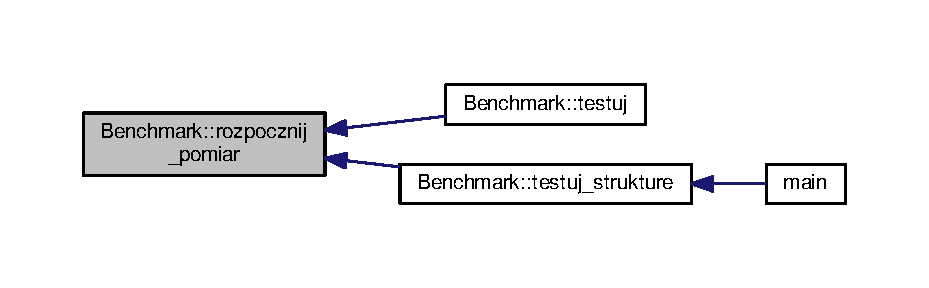
\includegraphics[width=350pt]{class_benchmark_a684ddcbdd22608838da1ad23f1fcc2ce_icgraph}
\end{center}
\end{figure}


\hypertarget{class_benchmark_ad2f9d4a8ee5a33de5261c2b2eff3d87a}{\index{Benchmark@{Benchmark}!testuj@{testuj}}
\index{testuj@{testuj}!Benchmark@{Benchmark}}
\subsubsection[{testuj}]{\setlength{\rightskip}{0pt plus 5cm}double Benchmark\-::testuj (
\begin{DoxyParamCaption}
\item[{{\bf Program} \&}]{program, }
\item[{char $\ast$}]{dane, }
\item[{int}]{ilosc\-\_\-danych, }
\item[{int}]{ilosc\-\_\-testow}
\end{DoxyParamCaption}
)}}\label{class_benchmark_ad2f9d4a8ee5a33de5261c2b2eff3d87a}
Dokonuje testow wybranego programu.


\begin{DoxyParams}[1]{Parametry}
\mbox{\tt in}  & {\em program} & \hyperlink{class_program}{Program} wybrany do testowania. \\
\hline
\mbox{\tt in}  & {\em dane} & Wskaznik na nazwe pliku z danymi. \\
\hline
\mbox{\tt in}  & {\em ilosc\-\_\-danych} & Ilosc danych, ktore chcemy pobrac do testu. \\
\hline
\mbox{\tt in}  & {\em ilosc\-\_\-testow} & Ilosc testow, jakie chcemy przeprowadzic.\\
\hline
\end{DoxyParams}
\begin{DoxyReturn}{Zwraca}
Metoda zwraca sredni czas wykonania programu dla podanych parametrow. 
\end{DoxyReturn}


Definicja w linii \hyperlink{benchmark_8cpp_source_l00017}{17} pliku \hyperlink{benchmark_8cpp_source}{benchmark.\-cpp}.



Oto graf wywołań dla tej funkcji\-:
\nopagebreak
\begin{figure}[H]
\begin{center}
\leavevmode
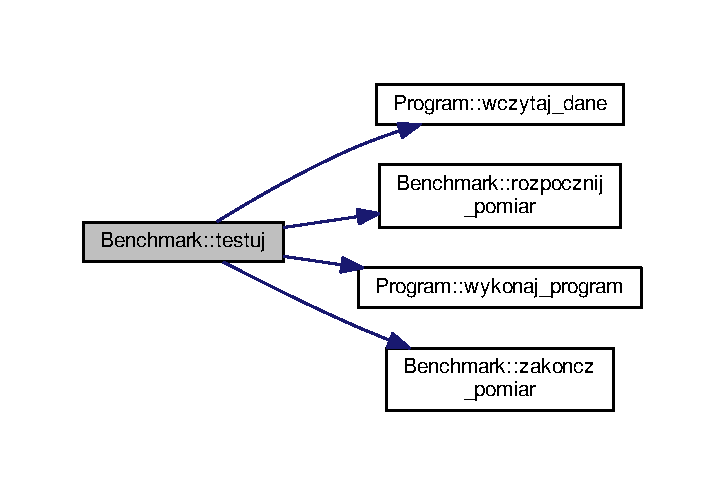
\includegraphics[width=348pt]{class_benchmark_ad2f9d4a8ee5a33de5261c2b2eff3d87a_cgraph}
\end{center}
\end{figure}




Oto graf wywoływań tej funkcji\-:
\nopagebreak
\begin{figure}[H]
\begin{center}
\leavevmode
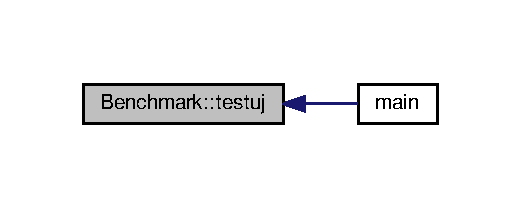
\includegraphics[width=250pt]{class_benchmark_ad2f9d4a8ee5a33de5261c2b2eff3d87a_icgraph}
\end{center}
\end{figure}


\hypertarget{class_benchmark_a3f4b4595a3d1145d238f5b3c8486d875}{\index{Benchmark@{Benchmark}!zakoncz\-\_\-pomiar@{zakoncz\-\_\-pomiar}}
\index{zakoncz\-\_\-pomiar@{zakoncz\-\_\-pomiar}!Benchmark@{Benchmark}}
\subsubsection[{zakoncz\-\_\-pomiar}]{\setlength{\rightskip}{0pt plus 5cm}void Benchmark\-::zakoncz\-\_\-pomiar (
\begin{DoxyParamCaption}
{}
\end{DoxyParamCaption}
)}}\label{class_benchmark_a3f4b4595a3d1145d238f5b3c8486d875}
Konczy pomiar czasu i zapisuje wartosc zmierzona w zmiennej czas\-\_\-pomiaru. 

Definicja w linii \hyperlink{benchmark_8cpp_source_l00011}{11} pliku \hyperlink{benchmark_8cpp_source}{benchmark.\-cpp}.



Oto graf wywoływań tej funkcji\-:
\nopagebreak
\begin{figure}[H]
\begin{center}
\leavevmode
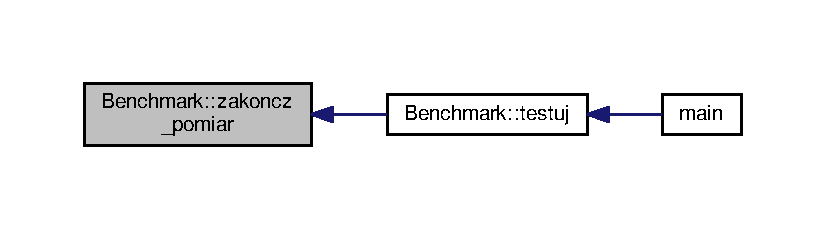
\includegraphics[width=350pt]{class_benchmark_a3f4b4595a3d1145d238f5b3c8486d875_icgraph}
\end{center}
\end{figure}




\subsection{Dokumentacja atrybutów składowych}
\hypertarget{class_benchmark_ab72b3cbe324970fd8c738f03718d52fc}{\index{Benchmark@{Benchmark}!czas\-\_\-pomiaru@{czas\-\_\-pomiaru}}
\index{czas\-\_\-pomiaru@{czas\-\_\-pomiaru}!Benchmark@{Benchmark}}
\subsubsection[{czas\-\_\-pomiaru}]{\setlength{\rightskip}{0pt plus 5cm}double Benchmark\-::czas\-\_\-pomiaru\hspace{0.3cm}{\ttfamily [private]}}}\label{class_benchmark_ab72b3cbe324970fd8c738f03718d52fc}
Przechowuje obliczony czas pojedynczego pomiaru (w ms) 

Definicja w linii \hyperlink{benchmark_8hh_source_l00037}{37} pliku \hyperlink{benchmark_8hh_source}{benchmark.\-hh}.

\hypertarget{class_benchmark_ab951e55dc4470926e0eb0761804f13bc}{\index{Benchmark@{Benchmark}!t1@{t1}}
\index{t1@{t1}!Benchmark@{Benchmark}}
\subsubsection[{t1}]{\setlength{\rightskip}{0pt plus 5cm}timeval Benchmark\-::t1\hspace{0.3cm}{\ttfamily [private]}}}\label{class_benchmark_ab951e55dc4470926e0eb0761804f13bc}
Zmienne przechowujace momenty rozpaczecia i zakonczenia pomiaru czasu. 

Definicja w linii \hyperlink{benchmark_8hh_source_l00030}{30} pliku \hyperlink{benchmark_8hh_source}{benchmark.\-hh}.

\hypertarget{class_benchmark_a2b145dd2458fea33d6df41f310058bec}{\index{Benchmark@{Benchmark}!t2@{t2}}
\index{t2@{t2}!Benchmark@{Benchmark}}
\subsubsection[{t2}]{\setlength{\rightskip}{0pt plus 5cm}timeval Benchmark\-::t2\hspace{0.3cm}{\ttfamily [private]}}}\label{class_benchmark_a2b145dd2458fea33d6df41f310058bec}


Definicja w linii \hyperlink{benchmark_8hh_source_l00030}{30} pliku \hyperlink{benchmark_8hh_source}{benchmark.\-hh}.



Dokumentacja dla tej klasy została wygenerowana z plików\-:\begin{DoxyCompactItemize}
\item 
\hyperlink{benchmark_8hh}{benchmark.\-hh}\item 
\hyperlink{benchmark_8cpp}{benchmark.\-cpp}\end{DoxyCompactItemize}

\hypertarget{class_lista}{\section{Dokumentacja szablonu klasy Lista$<$ type, type2 $>$}
\label{class_lista}\index{Lista$<$ type, type2 $>$@{Lista$<$ type, type2 $>$}}
}


{\ttfamily \#include $<$lista.\-hh$>$}



Diagram dziedziczenia dla Lista$<$ type, type2 $>$
\nopagebreak
\begin{figure}[H]
\begin{center}
\leavevmode
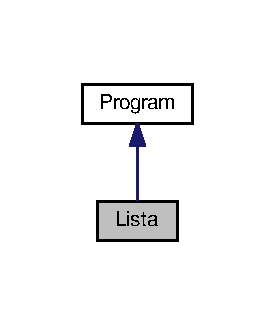
\includegraphics[width=184pt]{class_lista__inherit__graph}
\end{center}
\end{figure}


Diagram współpracy dla Lista$<$ type, type2 $>$\-:
\nopagebreak
\begin{figure}[H]
\begin{center}
\leavevmode
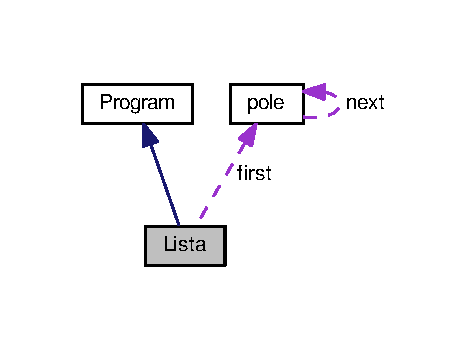
\includegraphics[width=285pt]{class_lista__coll__graph}
\end{center}
\end{figure}
\subsection*{Komponenty}
\begin{DoxyCompactItemize}
\item 
struct \hyperlink{struct_lista_1_1pole}{pole}
\begin{DoxyCompactList}\small\item\em Struktura pole. \end{DoxyCompactList}\end{DoxyCompactItemize}
\subsection*{Metody publiczne}
\begin{DoxyCompactItemize}
\item 
\hyperlink{class_lista_a43eba77afd8dcde8d1492bf8ca283319}{Lista} ()
\begin{DoxyCompactList}\small\item\em Konstruktor bezparametryczny. \end{DoxyCompactList}\item 
void \hyperlink{class_lista_a3b89123537e441b622630a1654afff3c}{push} (type x, type2 y)
\begin{DoxyCompactList}\small\item\em Metoda push. \end{DoxyCompactList}\item 
void \hyperlink{class_lista_aa0a993823fa462fbe6d6072a61f1a1f3}{push\-\_\-front} (type x, type2 y)
\begin{DoxyCompactList}\small\item\em Metoda push. \end{DoxyCompactList}\item 
void \hyperlink{class_lista_ac3c0760924a0cae03f837a581640d32b}{pop} ()
\begin{DoxyCompactList}\small\item\em Procedura pop. \end{DoxyCompactList}\item 
int \hyperlink{class_lista_a2951b209d8977cc61a570ce46fff1e82}{size} ()
\begin{DoxyCompactList}\small\item\em Metoda size. \end{DoxyCompactList}\item 
bool \hyperlink{class_lista_af74ba5fb933184e05ec9daf952f4cf86}{wykonaj\-\_\-program} (char $\ast$nazwa\-\_\-pliku, int ilosc\-\_\-danych)
\begin{DoxyCompactList}\small\item\em Metoda wykonaj\-\_\-program. \end{DoxyCompactList}\item 
void \hyperlink{class_lista_aee6110c6d9d5b36fe5342f2f8968d5ad}{wyczysc\-\_\-dane} (int ile)
\begin{DoxyCompactList}\small\item\em Metoda wyczysc\-\_\-dane. \end{DoxyCompactList}\item 
void \hyperlink{class_lista_aca842e81998c231283f8d82b3c17fbc8}{wyswietl} ()
\item 
void \hyperlink{class_lista_a234e4c9e70c2d71c281173a5348032d0}{wyswietl} (type key)
\item 
type2 \& \hyperlink{class_lista_a00136dbc6562f02884a8b27bf98e51d8}{daj} (type key)
\item 
void \hyperlink{class_lista_ac5309fa4e772c9de87abdd0a752bafad}{pop} (type key)
\begin{DoxyCompactList}\small\item\em Procedura pop. \end{DoxyCompactList}\end{DoxyCompactItemize}
\subsection*{Atrybuty publiczne}
\begin{DoxyCompactItemize}
\item 
\hyperlink{struct_lista_1_1pole}{pole} $\ast$ \hyperlink{class_lista_a7b19bc8c210d1bac9bb7608a638a8b27}{first}
\end{DoxyCompactItemize}
\subsection*{Dodatkowe Dziedziczone Składowe}


\subsection{Opis szczegółowy}
\subsubsection*{template$<$class type, class type2$>$class Lista$<$ type, type2 $>$}



Definicja w linii \hyperlink{lista_8hh_source_l00022}{22} pliku \hyperlink{lista_8hh_source}{lista.\-hh}.



\subsection{Dokumentacja konstruktora i destruktora}
\hypertarget{class_lista_a43eba77afd8dcde8d1492bf8ca283319}{\index{Lista@{Lista}!Lista@{Lista}}
\index{Lista@{Lista}!Lista@{Lista}}
\subsubsection[{Lista}]{\setlength{\rightskip}{0pt plus 5cm}template$<$class type, class type2$>$ {\bf Lista}$<$ type, type2 $>$\-::{\bf Lista} (
\begin{DoxyParamCaption}
{}
\end{DoxyParamCaption}
)\hspace{0.3cm}{\ttfamily [inline]}}}\label{class_lista_a43eba77afd8dcde8d1492bf8ca283319}
Ustawia poczatek listy na N\-U\-L\-L 

Definicja w linii \hyperlink{lista_8hh_source_l00044}{44} pliku \hyperlink{lista_8hh_source}{lista.\-hh}.



\subsection{Dokumentacja funkcji składowych}
\hypertarget{class_lista_a00136dbc6562f02884a8b27bf98e51d8}{\index{Lista@{Lista}!daj@{daj}}
\index{daj@{daj}!Lista@{Lista}}
\subsubsection[{daj}]{\setlength{\rightskip}{0pt plus 5cm}template$<$class type, class type2 $>$ type2 \& {\bf Lista}$<$ type, type2 $>$\-::daj (
\begin{DoxyParamCaption}
\item[{type}]{key}
\end{DoxyParamCaption}
)}}\label{class_lista_a00136dbc6562f02884a8b27bf98e51d8}


Definicja w linii \hyperlink{lista_8hh_source_l00238}{238} pliku \hyperlink{lista_8hh_source}{lista.\-hh}.

\hypertarget{class_lista_ac3c0760924a0cae03f837a581640d32b}{\index{Lista@{Lista}!pop@{pop}}
\index{pop@{pop}!Lista@{Lista}}
\subsubsection[{pop}]{\setlength{\rightskip}{0pt plus 5cm}template$<$class type , class type2 $>$ void {\bf Lista}$<$ type, type2 $>$\-::pop (
\begin{DoxyParamCaption}
{}
\end{DoxyParamCaption}
)}}\label{class_lista_ac3c0760924a0cae03f837a581640d32b}
Usuwa ostatni element listy. 

Definicja w linii \hyperlink{lista_8hh_source_l00178}{178} pliku \hyperlink{lista_8hh_source}{lista.\-hh}.

\hypertarget{class_lista_ac5309fa4e772c9de87abdd0a752bafad}{\index{Lista@{Lista}!pop@{pop}}
\index{pop@{pop}!Lista@{Lista}}
\subsubsection[{pop}]{\setlength{\rightskip}{0pt plus 5cm}template$<$class type, class type2 $>$ void {\bf Lista}$<$ type, type2 $>$\-::pop (
\begin{DoxyParamCaption}
\item[{type}]{key}
\end{DoxyParamCaption}
)}}\label{class_lista_ac5309fa4e772c9de87abdd0a752bafad}
Usuwa wszystkie elementy listy o podanej wartosci val1.


\begin{DoxyParams}[1]{Parametry}
\mbox{\tt in}  & {\em Wartosc} & val1 elementow do usuniecia \\
\hline
\end{DoxyParams}


Definicja w linii \hyperlink{lista_8hh_source_l00258}{258} pliku \hyperlink{lista_8hh_source}{lista.\-hh}.

\hypertarget{class_lista_a3b89123537e441b622630a1654afff3c}{\index{Lista@{Lista}!push@{push}}
\index{push@{push}!Lista@{Lista}}
\subsubsection[{push}]{\setlength{\rightskip}{0pt plus 5cm}template$<$class type, class type2$>$ void {\bf Lista}$<$ type, type2 $>$\-::push (
\begin{DoxyParamCaption}
\item[{type}]{x, }
\item[{type2}]{y}
\end{DoxyParamCaption}
)}}\label{class_lista_a3b89123537e441b622630a1654afff3c}
Dodaje podana wartosc na koniec listy.


\begin{DoxyParams}[1]{Parametry}
\mbox{\tt in}  & {\em x} & Wartosc, ktora chcemy dodac na koniec listy. \\
\hline
\end{DoxyParams}


Definicja w linii \hyperlink{lista_8hh_source_l00148}{148} pliku \hyperlink{lista_8hh_source}{lista.\-hh}.

\hypertarget{class_lista_aa0a993823fa462fbe6d6072a61f1a1f3}{\index{Lista@{Lista}!push\-\_\-front@{push\-\_\-front}}
\index{push\-\_\-front@{push\-\_\-front}!Lista@{Lista}}
\subsubsection[{push\-\_\-front}]{\setlength{\rightskip}{0pt plus 5cm}template$<$class type, class type2$>$ void {\bf Lista}$<$ type, type2 $>$\-::push\-\_\-front (
\begin{DoxyParamCaption}
\item[{type}]{x, }
\item[{type2}]{y}
\end{DoxyParamCaption}
)}}\label{class_lista_aa0a993823fa462fbe6d6072a61f1a1f3}
Dodaje podana wartosc na koniec listy.


\begin{DoxyParams}[1]{Parametry}
\mbox{\tt in}  & {\em x} & Wartosc, ktora chcemy dodac na poczatek listy. \\
\hline
\end{DoxyParams}


Definicja w linii \hyperlink{lista_8hh_source_l00164}{164} pliku \hyperlink{lista_8hh_source}{lista.\-hh}.

\hypertarget{class_lista_a2951b209d8977cc61a570ce46fff1e82}{\index{Lista@{Lista}!size@{size}}
\index{size@{size}!Lista@{Lista}}
\subsubsection[{size}]{\setlength{\rightskip}{0pt plus 5cm}template$<$class type , class type2 $>$ int {\bf Lista}$<$ type, type2 $>$\-::size (
\begin{DoxyParamCaption}
{}
\end{DoxyParamCaption}
)}}\label{class_lista_a2951b209d8977cc61a570ce46fff1e82}
Daje informacje o rozmiarze listy (liczbie jej elementow).

\begin{DoxyReturn}{Zwraca}
Rozmiar listy (liczba jej elementow) 
\end{DoxyReturn}


Definicja w linii \hyperlink{lista_8hh_source_l00200}{200} pliku \hyperlink{lista_8hh_source}{lista.\-hh}.

\hypertarget{class_lista_aee6110c6d9d5b36fe5342f2f8968d5ad}{\index{Lista@{Lista}!wyczysc\-\_\-dane@{wyczysc\-\_\-dane}}
\index{wyczysc\-\_\-dane@{wyczysc\-\_\-dane}!Lista@{Lista}}
\subsubsection[{wyczysc\-\_\-dane}]{\setlength{\rightskip}{0pt plus 5cm}template$<$class type , class type2 $>$ void {\bf Lista}$<$ type, type2 $>$\-::wyczysc\-\_\-dane (
\begin{DoxyParamCaption}
\item[{int}]{ile}
\end{DoxyParamCaption}
)\hspace{0.3cm}{\ttfamily [virtual]}}}\label{class_lista_aee6110c6d9d5b36fe5342f2f8968d5ad}
Usuwa zadana ilosc elementow listy za pomoca metody pop


\begin{DoxyParams}[1]{Parametry}
\mbox{\tt in}  & {\em ile} & Liczba elementow, ktore chcemy usunac. \\
\hline
\end{DoxyParams}


Implementuje \hyperlink{class_program_a4f26df1d57d90eeb7095e1ef2fe4c229}{Program}.



Definicja w linii \hyperlink{lista_8hh_source_l00218}{218} pliku \hyperlink{lista_8hh_source}{lista.\-hh}.

\hypertarget{class_lista_af74ba5fb933184e05ec9daf952f4cf86}{\index{Lista@{Lista}!wykonaj\-\_\-program@{wykonaj\-\_\-program}}
\index{wykonaj\-\_\-program@{wykonaj\-\_\-program}!Lista@{Lista}}
\subsubsection[{wykonaj\-\_\-program}]{\setlength{\rightskip}{0pt plus 5cm}template$<$class type , class type2 $>$ bool {\bf Lista}$<$ type, type2 $>$\-::wykonaj\-\_\-program (
\begin{DoxyParamCaption}
\item[{char $\ast$}]{nazwa\-\_\-pliku, }
\item[{int}]{ilosc\-\_\-danych}
\end{DoxyParamCaption}
)\hspace{0.3cm}{\ttfamily [virtual]}}}\label{class_lista_af74ba5fb933184e05ec9daf952f4cf86}
Wykonuje zadany program -\/ dodanie zadanej ilosci danych z pliku do listy za pomoca metody \hyperlink{class_lista_a3b89123537e441b622630a1654afff3c}{push()}


\begin{DoxyRetVals}{Zwracane wartości}
{\em T\-R\-U\-E} & Poprawnie wykonano program \\
\hline
{\em F\-A\-L\-S\-E} & Nie wczytano danych \\
\hline
\end{DoxyRetVals}


Implementuje \hyperlink{class_program_afc2ba31ffb01e8d2c6448a222fa02c8c}{Program}.



Definicja w linii \hyperlink{lista_8hh_source_l00214}{214} pliku \hyperlink{lista_8hh_source}{lista.\-hh}.

\hypertarget{class_lista_aca842e81998c231283f8d82b3c17fbc8}{\index{Lista@{Lista}!wyswietl@{wyswietl}}
\index{wyswietl@{wyswietl}!Lista@{Lista}}
\subsubsection[{wyswietl}]{\setlength{\rightskip}{0pt plus 5cm}template$<$class type, class type2$>$ void {\bf Lista}$<$ type, type2 $>$\-::wyswietl (
\begin{DoxyParamCaption}
{}
\end{DoxyParamCaption}
)\hspace{0.3cm}{\ttfamily [inline]}}}\label{class_lista_aca842e81998c231283f8d82b3c17fbc8}


Definicja w linii \hyperlink{lista_8hh_source_l00106}{106} pliku \hyperlink{lista_8hh_source}{lista.\-hh}.

\hypertarget{class_lista_a234e4c9e70c2d71c281173a5348032d0}{\index{Lista@{Lista}!wyswietl@{wyswietl}}
\index{wyswietl@{wyswietl}!Lista@{Lista}}
\subsubsection[{wyswietl}]{\setlength{\rightskip}{0pt plus 5cm}template$<$class type, class type2 $>$ void {\bf Lista}$<$ type, type2 $>$\-::wyswietl (
\begin{DoxyParamCaption}
\item[{type}]{key}
\end{DoxyParamCaption}
)}}\label{class_lista_a234e4c9e70c2d71c281173a5348032d0}


Definicja w linii \hyperlink{lista_8hh_source_l00223}{223} pliku \hyperlink{lista_8hh_source}{lista.\-hh}.



\subsection{Dokumentacja atrybutów składowych}
\hypertarget{class_lista_a7b19bc8c210d1bac9bb7608a638a8b27}{\index{Lista@{Lista}!first@{first}}
\index{first@{first}!Lista@{Lista}}
\subsubsection[{first}]{\setlength{\rightskip}{0pt plus 5cm}template$<$class type, class type2$>$ {\bf pole}$\ast$ {\bf Lista}$<$ type, type2 $>$\-::first}}\label{class_lista_a7b19bc8c210d1bac9bb7608a638a8b27}


Definicja w linii \hyperlink{lista_8hh_source_l00037}{37} pliku \hyperlink{lista_8hh_source}{lista.\-hh}.



Dokumentacja dla tej klasy została wygenerowana z pliku\-:\begin{DoxyCompactItemize}
\item 
\hyperlink{lista_8hh}{lista.\-hh}\end{DoxyCompactItemize}

\hypertarget{class_lista__tab}{\section{Dokumentacja klasy Lista\-\_\-tab}
\label{class_lista__tab}\index{Lista\-\_\-tab@{Lista\-\_\-tab}}
}


{\ttfamily \#include $<$lista\-\_\-tab.\-hh$>$}



Diagram dziedziczenia dla Lista\-\_\-tab\nopagebreak
\begin{figure}[H]
\begin{center}
\leavevmode
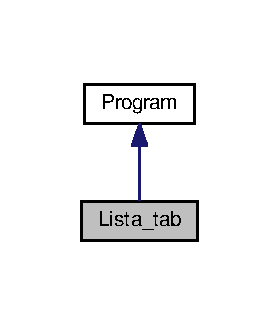
\includegraphics[width=134pt]{class_lista__tab__inherit__graph}
\end{center}
\end{figure}


Diagram współpracy dla Lista\-\_\-tab\-:\nopagebreak
\begin{figure}[H]
\begin{center}
\leavevmode
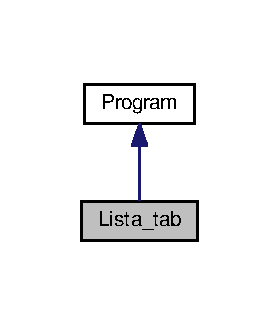
\includegraphics[width=134pt]{class_lista__tab__coll__graph}
\end{center}
\end{figure}
\subsection*{Metody publiczne}
\begin{DoxyCompactItemize}
\item 
\hyperlink{class_lista__tab_af10d3131eadfebb4df8abbe6379e6d7c}{Lista\-\_\-tab} ()
\begin{DoxyCompactList}\small\item\em Konstruktor bezparametryczny. \end{DoxyCompactList}\item 
\hyperlink{class_lista__tab_aaf55f952c14d2996c6f1e09acd718528}{$\sim$\-Lista\-\_\-tab} ()
\begin{DoxyCompactList}\small\item\em Destruktor. \end{DoxyCompactList}\item 
void \hyperlink{class_lista__tab_a800998768639b41b5be5c52ec4ccbda4}{push} (int x)
\begin{DoxyCompactList}\small\item\em Metoda push. \end{DoxyCompactList}\item 
void \hyperlink{class_lista__tab_affc42a7ffc6eda21076fc56eae38e980}{pop} ()
\begin{DoxyCompactList}\small\item\em Procedura pop. \end{DoxyCompactList}\item 
int \hyperlink{class_lista__tab_af092dd7943f7cd5ff407485f2991a1e4}{size} ()
\begin{DoxyCompactList}\small\item\em Metoda size. \end{DoxyCompactList}\item 
bool \hyperlink{class_lista__tab_ac9adc6ecc7348c5e1871b239c1313405}{wykonaj\-\_\-program} (char $\ast$nazwa\-\_\-pliku, int ilosc\-\_\-danych)
\begin{DoxyCompactList}\small\item\em Metoda wykonaj\-\_\-program. \end{DoxyCompactList}\item 
void \hyperlink{class_lista__tab_a506a6de79a600bac8316a6caf9878528}{wyczysc\-\_\-dane} (int ile)
\begin{DoxyCompactList}\small\item\em Metoda wyczysc\-\_\-dane. \end{DoxyCompactList}\item 
void \hyperlink{class_lista__tab_a409e9a4edbef4337980c7184b6cbfb63}{mergesort} (int beg, int end)
\begin{DoxyCompactList}\small\item\em Metoda mergesort. \end{DoxyCompactList}\item 
void \hyperlink{class_lista__tab_a34c4a75347b05d367d7d1b08fcbde095}{test} ()
\begin{DoxyCompactList}\small\item\em Metoda test. \end{DoxyCompactList}\end{DoxyCompactItemize}
\subsection*{Atrybuty publiczne}
\begin{DoxyCompactItemize}
\item 
int \hyperlink{class_lista__tab_a59e0425d896070457d1f3456b91842fd}{rozmiar}
\begin{DoxyCompactList}\small\item\em Aktualny rozmiar tablicy. \end{DoxyCompactList}\item 
int \hyperlink{class_lista__tab_afd2c6ba3ae15e658890641b188c7ed39}{iterator}
\begin{DoxyCompactList}\small\item\em Iterator, zawierajacy informacje o liczbie elementow w tablicy. \end{DoxyCompactList}\item 
int $\ast$ \hyperlink{class_lista__tab_a123dfb670e5a5592e512c41cc4faf14e}{tab}
\begin{DoxyCompactList}\small\item\em Wskaznik na dynamicznie alokowana tablice z danymi. \end{DoxyCompactList}\end{DoxyCompactItemize}
\subsection*{Dodatkowe Dziedziczone Składowe}


\subsection{Opis szczegółowy}


Definicja w linii \hyperlink{lista__tab_8hh_source_l00012}{12} pliku \hyperlink{lista__tab_8hh_source}{lista\-\_\-tab.\-hh}.



\subsection{Dokumentacja konstruktora i destruktora}
\hypertarget{class_lista__tab_af10d3131eadfebb4df8abbe6379e6d7c}{\index{Lista\-\_\-tab@{Lista\-\_\-tab}!Lista\-\_\-tab@{Lista\-\_\-tab}}
\index{Lista\-\_\-tab@{Lista\-\_\-tab}!Lista_tab@{Lista\-\_\-tab}}
\subsubsection[{Lista\-\_\-tab}]{\setlength{\rightskip}{0pt plus 5cm}Lista\-\_\-tab\-::\-Lista\-\_\-tab (
\begin{DoxyParamCaption}
{}
\end{DoxyParamCaption}
)\hspace{0.3cm}{\ttfamily [inline]}}}\label{class_lista__tab_af10d3131eadfebb4df8abbe6379e6d7c}
Ustawia poczatek listy na N\-U\-L\-L 

Definicja w linii \hyperlink{lista__tab_8hh_source_l00031}{31} pliku \hyperlink{lista__tab_8hh_source}{lista\-\_\-tab.\-hh}.

\hypertarget{class_lista__tab_aaf55f952c14d2996c6f1e09acd718528}{\index{Lista\-\_\-tab@{Lista\-\_\-tab}!$\sim$\-Lista\-\_\-tab@{$\sim$\-Lista\-\_\-tab}}
\index{$\sim$\-Lista\-\_\-tab@{$\sim$\-Lista\-\_\-tab}!Lista_tab@{Lista\-\_\-tab}}
\subsubsection[{$\sim$\-Lista\-\_\-tab}]{\setlength{\rightskip}{0pt plus 5cm}Lista\-\_\-tab\-::$\sim$\-Lista\-\_\-tab (
\begin{DoxyParamCaption}
{}
\end{DoxyParamCaption}
)\hspace{0.3cm}{\ttfamily [inline]}}}\label{class_lista__tab_aaf55f952c14d2996c6f1e09acd718528}
Usuwa dynamicznie utworzona tablice danych oraz przypisuje wskaznikowi wartosc N\-U\-L\-L. 

Definicja w linii \hyperlink{lista__tab_8hh_source_l00043}{43} pliku \hyperlink{lista__tab_8hh_source}{lista\-\_\-tab.\-hh}.



\subsection{Dokumentacja funkcji składowych}
\hypertarget{class_lista__tab_a409e9a4edbef4337980c7184b6cbfb63}{\index{Lista\-\_\-tab@{Lista\-\_\-tab}!mergesort@{mergesort}}
\index{mergesort@{mergesort}!Lista_tab@{Lista\-\_\-tab}}
\subsubsection[{mergesort}]{\setlength{\rightskip}{0pt plus 5cm}void Lista\-\_\-tab\-::mergesort (
\begin{DoxyParamCaption}
\item[{int}]{beg, }
\item[{int}]{end}
\end{DoxyParamCaption}
)}}\label{class_lista__tab_a409e9a4edbef4337980c7184b6cbfb63}
Dokonuje sortowania tablicy przez scalanie


\begin{DoxyParams}[1]{Parametry}
\mbox{\tt in}  & {\em beg} & Początek obszaru sortowania \\
\hline
\mbox{\tt in}  & {\em end} & Koniec obszaru sortowania \\
\hline
\end{DoxyParams}


Definicja w linii \hyperlink{lista__tab_8cpp_source_l00100}{100} pliku \hyperlink{lista__tab_8cpp_source}{lista\-\_\-tab.\-cpp}.



Oto graf wywoływań tej funkcji\-:
\nopagebreak
\begin{figure}[H]
\begin{center}
\leavevmode
\includegraphics[width=302pt]{class_lista__tab_a409e9a4edbef4337980c7184b6cbfb63_icgraph}
\end{center}
\end{figure}


\hypertarget{class_lista__tab_affc42a7ffc6eda21076fc56eae38e980}{\index{Lista\-\_\-tab@{Lista\-\_\-tab}!pop@{pop}}
\index{pop@{pop}!Lista_tab@{Lista\-\_\-tab}}
\subsubsection[{pop}]{\setlength{\rightskip}{0pt plus 5cm}void Lista\-\_\-tab\-::pop (
\begin{DoxyParamCaption}
{}
\end{DoxyParamCaption}
)}}\label{class_lista__tab_affc42a7ffc6eda21076fc56eae38e980}
Usuwa ostatni element listy. 

Definicja w linii \hyperlink{lista__tab_8cpp_source_l00056}{56} pliku \hyperlink{lista__tab_8cpp_source}{lista\-\_\-tab.\-cpp}.

\hypertarget{class_lista__tab_a800998768639b41b5be5c52ec4ccbda4}{\index{Lista\-\_\-tab@{Lista\-\_\-tab}!push@{push}}
\index{push@{push}!Lista_tab@{Lista\-\_\-tab}}
\subsubsection[{push}]{\setlength{\rightskip}{0pt plus 5cm}void Lista\-\_\-tab\-::push (
\begin{DoxyParamCaption}
\item[{int}]{x}
\end{DoxyParamCaption}
)}}\label{class_lista__tab_a800998768639b41b5be5c52ec4ccbda4}
Dodaje podana wartosc na koniec listy. Do wyboru 2 metody push -\/ po osiagnieciu maksymalnego rozmiaru tablicy, jedna z nich zwieksza rozmiar tablicy o 1, a druga podwaja aktualny rozmiar tablicy. Wyboru metody nalezy dokonac poprzed odkomentowanie odpowiedniej metody w pliku .cpp.


\begin{DoxyParams}[1]{Parametry}
\mbox{\tt in}  & {\em x} & Wartosc, ktora chcemy dodac na koniec listy. \\
\hline
\end{DoxyParams}


Definicja w linii \hyperlink{lista__tab_8cpp_source_l00032}{32} pliku \hyperlink{lista__tab_8cpp_source}{lista\-\_\-tab.\-cpp}.



Oto graf wywoływań tej funkcji\-:
\nopagebreak
\begin{figure}[H]
\begin{center}
\leavevmode
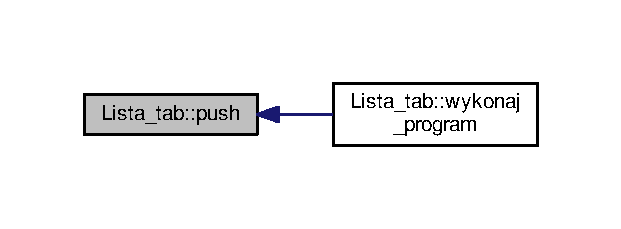
\includegraphics[width=350pt]{class_lista__tab_a800998768639b41b5be5c52ec4ccbda4_icgraph}
\end{center}
\end{figure}


\hypertarget{class_lista__tab_af092dd7943f7cd5ff407485f2991a1e4}{\index{Lista\-\_\-tab@{Lista\-\_\-tab}!size@{size}}
\index{size@{size}!Lista_tab@{Lista\-\_\-tab}}
\subsubsection[{size}]{\setlength{\rightskip}{0pt plus 5cm}int Lista\-\_\-tab\-::size (
\begin{DoxyParamCaption}
{}
\end{DoxyParamCaption}
)}}\label{class_lista__tab_af092dd7943f7cd5ff407485f2991a1e4}
Daje informacje o rozmiarze listy (liczbie jej elementow).

\begin{DoxyReturn}{Zwraca}
Rozmiar listy (liczba jej elementow) 
\end{DoxyReturn}


Definicja w linii \hyperlink{lista__tab_8cpp_source_l00073}{73} pliku \hyperlink{lista__tab_8cpp_source}{lista\-\_\-tab.\-cpp}.

\hypertarget{class_lista__tab_a34c4a75347b05d367d7d1b08fcbde095}{\index{Lista\-\_\-tab@{Lista\-\_\-tab}!test@{test}}
\index{test@{test}!Lista_tab@{Lista\-\_\-tab}}
\subsubsection[{test}]{\setlength{\rightskip}{0pt plus 5cm}void Lista\-\_\-tab\-::test (
\begin{DoxyParamCaption}
{}
\end{DoxyParamCaption}
)\hspace{0.3cm}{\ttfamily [inline]}, {\ttfamily [virtual]}}}\label{class_lista__tab_a34c4a75347b05d367d7d1b08fcbde095}
Wykonuje sortowanie przez scalanie 

Reimplementowana z \hyperlink{class_program_ae866e995ea153f83031107c194f604e5}{Program}.



Definicja w linii \hyperlink{lista__tab_8hh_source_l00107}{107} pliku \hyperlink{lista__tab_8hh_source}{lista\-\_\-tab.\-hh}.



Oto graf wywołań dla tej funkcji\-:
\nopagebreak
\begin{figure}[H]
\begin{center}
\leavevmode
\includegraphics[width=302pt]{class_lista__tab_a34c4a75347b05d367d7d1b08fcbde095_cgraph}
\end{center}
\end{figure}


\hypertarget{class_lista__tab_a506a6de79a600bac8316a6caf9878528}{\index{Lista\-\_\-tab@{Lista\-\_\-tab}!wyczysc\-\_\-dane@{wyczysc\-\_\-dane}}
\index{wyczysc\-\_\-dane@{wyczysc\-\_\-dane}!Lista_tab@{Lista\-\_\-tab}}
\subsubsection[{wyczysc\-\_\-dane}]{\setlength{\rightskip}{0pt plus 5cm}void Lista\-\_\-tab\-::wyczysc\-\_\-dane (
\begin{DoxyParamCaption}
\item[{int}]{ile}
\end{DoxyParamCaption}
)\hspace{0.3cm}{\ttfamily [virtual]}}}\label{class_lista__tab_a506a6de79a600bac8316a6caf9878528}
Usuwa zadana ilosc elementow listy za pomoca metody pop


\begin{DoxyParams}[1]{Parametry}
\mbox{\tt in}  & {\em ile} & Liczba elementow, ktore chcemy usunac. \\
\hline
\end{DoxyParams}


Implementuje \hyperlink{class_program_a4f26df1d57d90eeb7095e1ef2fe4c229}{Program}.



Definicja w linii \hyperlink{lista__tab_8cpp_source_l00093}{93} pliku \hyperlink{lista__tab_8cpp_source}{lista\-\_\-tab.\-cpp}.

\hypertarget{class_lista__tab_ac9adc6ecc7348c5e1871b239c1313405}{\index{Lista\-\_\-tab@{Lista\-\_\-tab}!wykonaj\-\_\-program@{wykonaj\-\_\-program}}
\index{wykonaj\-\_\-program@{wykonaj\-\_\-program}!Lista_tab@{Lista\-\_\-tab}}
\subsubsection[{wykonaj\-\_\-program}]{\setlength{\rightskip}{0pt plus 5cm}bool Lista\-\_\-tab\-::wykonaj\-\_\-program (
\begin{DoxyParamCaption}
\item[{char $\ast$}]{nazwa\-\_\-pliku, }
\item[{int}]{ilosc\-\_\-danych}
\end{DoxyParamCaption}
)\hspace{0.3cm}{\ttfamily [virtual]}}}\label{class_lista__tab_ac9adc6ecc7348c5e1871b239c1313405}
Wykonuje zadany program -\/ dodanie zadanej ilosci danych z pliku do listy za pomoca metody \hyperlink{class_lista__tab_a800998768639b41b5be5c52ec4ccbda4}{push()}


\begin{DoxyRetVals}{Zwracane wartości}
{\em T\-R\-U\-E} & Poprawnie wykonano program \\
\hline
{\em F\-A\-L\-S\-E} & Nie wczytano danych \\
\hline
\end{DoxyRetVals}


Implementuje \hyperlink{class_program_afc2ba31ffb01e8d2c6448a222fa02c8c}{Program}.



Definicja w linii \hyperlink{lista__tab_8cpp_source_l00077}{77} pliku \hyperlink{lista__tab_8cpp_source}{lista\-\_\-tab.\-cpp}.



Oto graf wywołań dla tej funkcji\-:\nopagebreak
\begin{figure}[H]
\begin{center}
\leavevmode
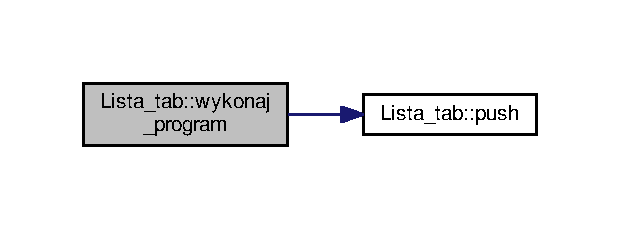
\includegraphics[width=298pt]{class_lista__tab_ac9adc6ecc7348c5e1871b239c1313405_cgraph}
\end{center}
\end{figure}




Oto graf wywoływań tej funkcji\-:
\nopagebreak
\begin{figure}[H]
\begin{center}
\leavevmode
\includegraphics[width=252pt]{class_lista__tab_ac9adc6ecc7348c5e1871b239c1313405_icgraph}
\end{center}
\end{figure}




\subsection{Dokumentacja atrybutów składowych}
\hypertarget{class_lista__tab_afd2c6ba3ae15e658890641b188c7ed39}{\index{Lista\-\_\-tab@{Lista\-\_\-tab}!iterator@{iterator}}
\index{iterator@{iterator}!Lista_tab@{Lista\-\_\-tab}}
\subsubsection[{iterator}]{\setlength{\rightskip}{0pt plus 5cm}int Lista\-\_\-tab\-::iterator}}\label{class_lista__tab_afd2c6ba3ae15e658890641b188c7ed39}


Definicja w linii \hyperlink{lista__tab_8hh_source_l00020}{20} pliku \hyperlink{lista__tab_8hh_source}{lista\-\_\-tab.\-hh}.

\hypertarget{class_lista__tab_a59e0425d896070457d1f3456b91842fd}{\index{Lista\-\_\-tab@{Lista\-\_\-tab}!rozmiar@{rozmiar}}
\index{rozmiar@{rozmiar}!Lista_tab@{Lista\-\_\-tab}}
\subsubsection[{rozmiar}]{\setlength{\rightskip}{0pt plus 5cm}int Lista\-\_\-tab\-::rozmiar}}\label{class_lista__tab_a59e0425d896070457d1f3456b91842fd}


Definicja w linii \hyperlink{lista__tab_8hh_source_l00016}{16} pliku \hyperlink{lista__tab_8hh_source}{lista\-\_\-tab.\-hh}.

\hypertarget{class_lista__tab_a123dfb670e5a5592e512c41cc4faf14e}{\index{Lista\-\_\-tab@{Lista\-\_\-tab}!tab@{tab}}
\index{tab@{tab}!Lista_tab@{Lista\-\_\-tab}}
\subsubsection[{tab}]{\setlength{\rightskip}{0pt plus 5cm}int$\ast$ Lista\-\_\-tab\-::tab}}\label{class_lista__tab_a123dfb670e5a5592e512c41cc4faf14e}


Definicja w linii \hyperlink{lista__tab_8hh_source_l00024}{24} pliku \hyperlink{lista__tab_8hh_source}{lista\-\_\-tab.\-hh}.



Dokumentacja dla tej klasy została wygenerowana z plików\-:\begin{DoxyCompactItemize}
\item 
\hyperlink{lista__tab_8hh}{lista\-\_\-tab.\-hh}\item 
\hyperlink{lista__tab_8cpp}{lista\-\_\-tab.\-cpp}\end{DoxyCompactItemize}

\input{struct_lista_1_1pole}
\hypertarget{class_program}{\section{Dokumentacja klasy Program}
\label{class_program}\index{Program@{Program}}
}


Modeluje klase \hyperlink{class_program}{Program}.  




{\ttfamily \#include $<$program.\-hh$>$}



Diagram dziedziczenia dla Program
\nopagebreak
\begin{figure}[H]
\begin{center}
\leavevmode
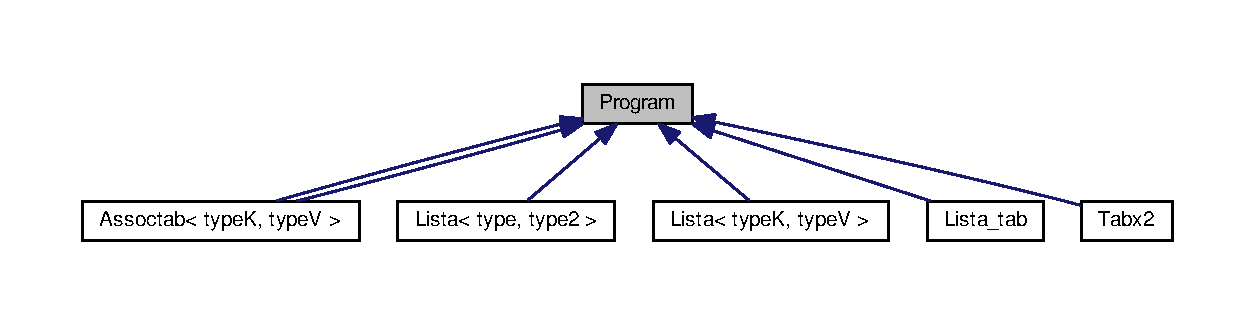
\includegraphics[width=350pt]{class_program__inherit__graph}
\end{center}
\end{figure}
\subsection*{Metody publiczne}
\begin{DoxyCompactItemize}
\item 
int \hyperlink{class_program_a4fb9c2979a0dca1e14c75f4cc461bebd}{get\-Rozmiar\-\_\-tab} ()
\begin{DoxyCompactList}\small\item\em Akcesor get\-Rozmiar\-\_\-tab. \end{DoxyCompactList}\item 
\hyperlink{class_program_aaefaa0df08f3484476fc4d61e97acbdc}{Program} ()
\begin{DoxyCompactList}\small\item\em Konstruktor bezparametryczny. \end{DoxyCompactList}\item 
\hyperlink{class_program_a986aef1c50e1d338a3315a47ba6df549}{$\sim$\-Program} ()
\begin{DoxyCompactList}\small\item\em Destruktor. \end{DoxyCompactList}\item 
bool \hyperlink{class_program_a618d9d6e3255ca5ff3d65de0385c6d46}{wczytaj\-\_\-dane} (char $\ast$nazwa\-\_\-pliku)
\begin{DoxyCompactList}\small\item\em Metoda wczytaj\-\_\-dane. \end{DoxyCompactList}\item 
bool \hyperlink{class_program_a6bfc0c61a365d212dbb73e95034185c1}{wczytaj\-\_\-dane} (char $\ast$nazwa\-\_\-pliku, int ile\-\_\-danych)
\begin{DoxyCompactList}\small\item\em Metoda wczytaj\-\_\-dane. \end{DoxyCompactList}\item 
bool \hyperlink{class_program_a0a0d555a69e791820a70000375462e32}{zapisz\-\_\-dane} (char $\ast$nazwa\-\_\-pliku)
\item 
void \hyperlink{class_program_ac939bc41859b867dd631163f6540573f}{wyswietl\-\_\-dane} ()
\begin{DoxyCompactList}\small\item\em Procedura wyswietl\-\_\-dane. \end{DoxyCompactList}\item 
virtual bool \hyperlink{class_program_ac396401ba5cade863d0e6acb727bec4e}{wykonaj\-\_\-program} ()
\begin{DoxyCompactList}\small\item\em Wirtualna metoda wykonaj\-\_\-program. \end{DoxyCompactList}\item 
virtual bool \hyperlink{class_program_afc2ba31ffb01e8d2c6448a222fa02c8c}{wykonaj\-\_\-program} (char $\ast$nazwa\-\_\-pliku, int ilosc\-\_\-danych)=0
\item 
virtual void \hyperlink{class_program_a4f26df1d57d90eeb7095e1ef2fe4c229}{wyczysc\-\_\-dane} (int ile)=0
\end{DoxyCompactItemize}
\subsection*{Atrybuty chronione}
\begin{DoxyCompactItemize}
\item 
int \hyperlink{class_program_a3b5a10104019b9daa23ce4a5f5533820}{rozmiar\-\_\-tab}
\begin{DoxyCompactList}\small\item\em Zmiena rozmiar\-\_\-tab. \end{DoxyCompactList}\item 
int $\ast$ \hyperlink{class_program_ac72268c925315098b1632cc97d0f818a}{tab}
\begin{DoxyCompactList}\small\item\em Zmienna tablica. \end{DoxyCompactList}\item 
ifstream \hyperlink{class_program_aac2f72538e24e533c327fe5546a59210}{plik\-\_\-we}
\begin{DoxyCompactList}\small\item\em Zmienna plik\-\_\-we. \end{DoxyCompactList}\item 
ofstream \hyperlink{class_program_a59c1761a5ea875b3d5a4678928f3a1de}{plik\-\_\-wy}
\begin{DoxyCompactList}\small\item\em Zmienna plik\-\_\-wy. \end{DoxyCompactList}\end{DoxyCompactItemize}


\subsection{Opis szczegółowy}
Klasa \hyperlink{class_program}{Program} zawiera zmienne oraz metody wspolne dla wszystkich programow. Sa one zwiazane z przechowywaniem i obsluga danych. 

Definicja w linii \hyperlink{program_8hh_source_l00022}{22} pliku \hyperlink{program_8hh_source}{program.\-hh}.



\subsection{Dokumentacja konstruktora i destruktora}
\hypertarget{class_program_aaefaa0df08f3484476fc4d61e97acbdc}{\index{Program@{Program}!Program@{Program}}
\index{Program@{Program}!Program@{Program}}
\subsubsection[{Program}]{\setlength{\rightskip}{0pt plus 5cm}Program\-::\-Program (
\begin{DoxyParamCaption}
{}
\end{DoxyParamCaption}
)\hspace{0.3cm}{\ttfamily [inline]}}}\label{class_program_aaefaa0df08f3484476fc4d61e97acbdc}
Przypisuje domyslna wartosc 0 dla rozmiaru tablicy danych oraz N\-U\-L\-L dla wskaznika. 

Definicja w linii \hyperlink{program_8hh_source_l00071}{71} pliku \hyperlink{program_8hh_source}{program.\-hh}.

\hypertarget{class_program_a986aef1c50e1d338a3315a47ba6df549}{\index{Program@{Program}!$\sim$\-Program@{$\sim$\-Program}}
\index{$\sim$\-Program@{$\sim$\-Program}!Program@{Program}}
\subsubsection[{$\sim$\-Program}]{\setlength{\rightskip}{0pt plus 5cm}Program\-::$\sim$\-Program (
\begin{DoxyParamCaption}
{}
\end{DoxyParamCaption}
)\hspace{0.3cm}{\ttfamily [inline]}}}\label{class_program_a986aef1c50e1d338a3315a47ba6df549}
Usuwa dynamicznie utworzona tablice danych oraz przypisuje wskaznikowi wartosc N\-U\-L\-L. 

Definicja w linii \hyperlink{program_8hh_source_l00079}{79} pliku \hyperlink{program_8hh_source}{program.\-hh}.



\subsection{Dokumentacja funkcji składowych}
\hypertarget{class_program_a4fb9c2979a0dca1e14c75f4cc461bebd}{\index{Program@{Program}!get\-Rozmiar\-\_\-tab@{get\-Rozmiar\-\_\-tab}}
\index{get\-Rozmiar\-\_\-tab@{get\-Rozmiar\-\_\-tab}!Program@{Program}}
\subsubsection[{get\-Rozmiar\-\_\-tab}]{\setlength{\rightskip}{0pt plus 5cm}int Program\-::get\-Rozmiar\-\_\-tab (
\begin{DoxyParamCaption}
{}
\end{DoxyParamCaption}
)\hspace{0.3cm}{\ttfamily [inline]}}}\label{class_program_a4fb9c2979a0dca1e14c75f4cc461bebd}
Metoda dajaca mozliwosc odczytu rozmiaru tablicy. 

Definicja w linii \hyperlink{program_8hh_source_l00063}{63} pliku \hyperlink{program_8hh_source}{program.\-hh}.

\hypertarget{class_program_a618d9d6e3255ca5ff3d65de0385c6d46}{\index{Program@{Program}!wczytaj\-\_\-dane@{wczytaj\-\_\-dane}}
\index{wczytaj\-\_\-dane@{wczytaj\-\_\-dane}!Program@{Program}}
\subsubsection[{wczytaj\-\_\-dane}]{\setlength{\rightskip}{0pt plus 5cm}bool Program\-::wczytaj\-\_\-dane (
\begin{DoxyParamCaption}
\item[{char $\ast$}]{nazwa\-\_\-pliku}
\end{DoxyParamCaption}
)}}\label{class_program_a618d9d6e3255ca5ff3d65de0385c6d46}
Wczytuje dane z pliku. W pierwszej linii pliku musi znajdowac sie informacja o ilosci wczytywanych danych, dane w kolejnych liniach\-: ilosc\-\_\-danych dana1 dana2 ...


\begin{DoxyParams}[1]{Parametry}
\mbox{\tt in}  & {\em nazwa\-\_\-pliku} & Wskaznik do nazwy pliku do wczytania.\\
\hline
\end{DoxyParams}

\begin{DoxyRetVals}{Zwracane wartości}
{\em T\-R\-U\-E} & Poprawnie wczytano plik. \\
\hline
{\em F\-A\-L\-S\-E} & Blad podczas wczytywania pliku. \\
\hline
\end{DoxyRetVals}


Definicja w linii \hyperlink{program_8cpp_source_l00008}{8} pliku \hyperlink{program_8cpp_source}{program.\-cpp}.



Oto graf wywoływań tej funkcji\-:\nopagebreak
\begin{figure}[H]
\begin{center}
\leavevmode
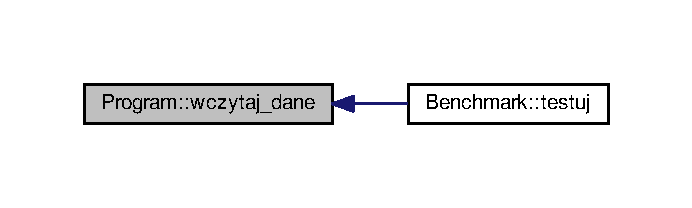
\includegraphics[width=332pt]{class_program_a618d9d6e3255ca5ff3d65de0385c6d46_icgraph}
\end{center}
\end{figure}


\hypertarget{class_program_a6bfc0c61a365d212dbb73e95034185c1}{\index{Program@{Program}!wczytaj\-\_\-dane@{wczytaj\-\_\-dane}}
\index{wczytaj\-\_\-dane@{wczytaj\-\_\-dane}!Program@{Program}}
\subsubsection[{wczytaj\-\_\-dane}]{\setlength{\rightskip}{0pt plus 5cm}bool Program\-::wczytaj\-\_\-dane (
\begin{DoxyParamCaption}
\item[{char $\ast$}]{nazwa\-\_\-pliku, }
\item[{int}]{ile\-\_\-danych}
\end{DoxyParamCaption}
)}}\label{class_program_a6bfc0c61a365d212dbb73e95034185c1}
Wczytuje okreslona liczbe danych z pliku. W pierwszej linii pliku musi znajdowac sie informacja o ilosci wczytywanych danych, dane w kolejnych liniach\-: ilosc\-\_\-danych dana1 dana2 ...


\begin{DoxyParams}[1]{Parametry}
\mbox{\tt in}  & {\em nazwa\-\_\-pliku} & Wskaznik do nazwy pliku do wczytania. \\
\hline
\mbox{\tt in}  & {\em ile\-\_\-danych} & Ilosc danych, jakie chcemy wczytac.\\
\hline
\end{DoxyParams}

\begin{DoxyRetVals}{Zwracane wartości}
{\em T\-R\-U\-E} & Poprawnie wczytano plik. \\
\hline
{\em F\-A\-L\-S\-E} & Blad podczas wczytywania pliku. \\
\hline
\end{DoxyRetVals}


Definicja w linii \hyperlink{program_8cpp_source_l00026}{26} pliku \hyperlink{program_8cpp_source}{program.\-cpp}.

\hypertarget{class_program_a4f26df1d57d90eeb7095e1ef2fe4c229}{\index{Program@{Program}!wyczysc\-\_\-dane@{wyczysc\-\_\-dane}}
\index{wyczysc\-\_\-dane@{wyczysc\-\_\-dane}!Program@{Program}}
\subsubsection[{wyczysc\-\_\-dane}]{\setlength{\rightskip}{0pt plus 5cm}virtual void Program\-::wyczysc\-\_\-dane (
\begin{DoxyParamCaption}
\item[{int}]{ile}
\end{DoxyParamCaption}
)\hspace{0.3cm}{\ttfamily [pure virtual]}}}\label{class_program_a4f26df1d57d90eeb7095e1ef2fe4c229}


Implementowany w \hyperlink{class_lista__tab_a506a6de79a600bac8316a6caf9878528}{Lista\-\_\-tab}, \hyperlink{class_lista_af73c0c1eba31c0d82d107d57e99fc3d7}{Lista}, \hyperlink{class_kolejka_aaf67b4be89eaa07ebd9cbae057dc2b0d}{Kolejka} i \hyperlink{class_stos_aa54f9d021e324f5a204dbc8193dd9a6e}{Stos}.



Oto graf wywoływań tej funkcji\-:\nopagebreak
\begin{figure}[H]
\begin{center}
\leavevmode
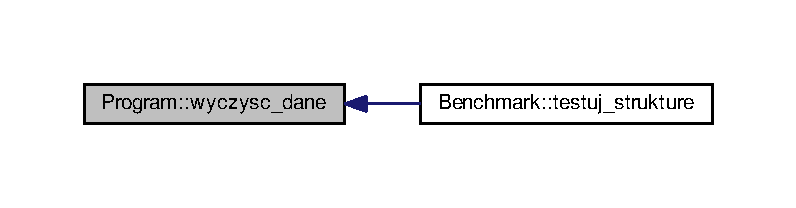
\includegraphics[width=350pt]{class_program_a4f26df1d57d90eeb7095e1ef2fe4c229_icgraph}
\end{center}
\end{figure}


\hypertarget{class_program_ac396401ba5cade863d0e6acb727bec4e}{\index{Program@{Program}!wykonaj\-\_\-program@{wykonaj\-\_\-program}}
\index{wykonaj\-\_\-program@{wykonaj\-\_\-program}!Program@{Program}}
\subsubsection[{wykonaj\-\_\-program}]{\setlength{\rightskip}{0pt plus 5cm}bool Program\-::wykonaj\-\_\-program (
\begin{DoxyParamCaption}
{}
\end{DoxyParamCaption}
)\hspace{0.3cm}{\ttfamily [virtual]}}}\label{class_program_ac396401ba5cade863d0e6acb727bec4e}
Wykonuje program na zadanej liczbie danych. 

Reimplementowana w \hyperlink{class_tabx2_a30db6636cba36a354443ec5f101fd188}{Tabx2}.



Definicja w linii \hyperlink{program_8cpp_source_l00067}{67} pliku \hyperlink{program_8cpp_source}{program.\-cpp}.



Oto graf wywoływań tej funkcji\-:\nopagebreak
\begin{figure}[H]
\begin{center}
\leavevmode
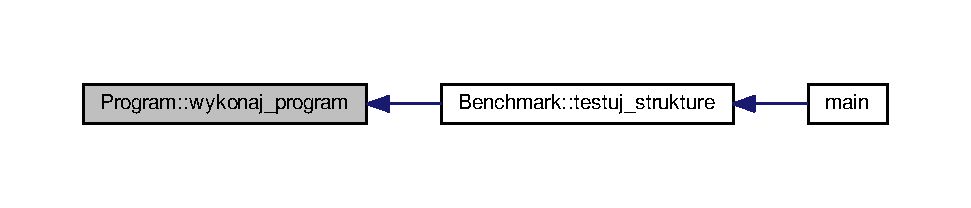
\includegraphics[width=350pt]{class_program_ac396401ba5cade863d0e6acb727bec4e_icgraph}
\end{center}
\end{figure}


\hypertarget{class_program_afc2ba31ffb01e8d2c6448a222fa02c8c}{\index{Program@{Program}!wykonaj\-\_\-program@{wykonaj\-\_\-program}}
\index{wykonaj\-\_\-program@{wykonaj\-\_\-program}!Program@{Program}}
\subsubsection[{wykonaj\-\_\-program}]{\setlength{\rightskip}{0pt plus 5cm}virtual bool Program\-::wykonaj\-\_\-program (
\begin{DoxyParamCaption}
\item[{char $\ast$}]{nazwa\-\_\-pliku, }
\item[{int}]{ilosc\-\_\-danych}
\end{DoxyParamCaption}
)\hspace{0.3cm}{\ttfamily [pure virtual]}}}\label{class_program_afc2ba31ffb01e8d2c6448a222fa02c8c}


Implementowany w \hyperlink{class_lista__tab_ac9adc6ecc7348c5e1871b239c1313405}{Lista\-\_\-tab}, \hyperlink{class_lista_a39367fb8f22f8bb34ba65bcc37f522bf}{Lista}, \hyperlink{class_kolejka_af849bac74dd62a28df378ed3f95b622e}{Kolejka} i \hyperlink{class_stos_a7b9d5405298070fa7cbd3389a99dbcc8}{Stos}.

\hypertarget{class_program_ac939bc41859b867dd631163f6540573f}{\index{Program@{Program}!wyswietl\-\_\-dane@{wyswietl\-\_\-dane}}
\index{wyswietl\-\_\-dane@{wyswietl\-\_\-dane}!Program@{Program}}
\subsubsection[{wyswietl\-\_\-dane}]{\setlength{\rightskip}{0pt plus 5cm}void Program\-::wyswietl\-\_\-dane (
\begin{DoxyParamCaption}
{}
\end{DoxyParamCaption}
)}}\label{class_program_ac939bc41859b867dd631163f6540573f}
Wypisuje wczytane dane jedna pod druga na standardowy strumien wyjscia. 

Definicja w linii \hyperlink{program_8cpp_source_l00062}{62} pliku \hyperlink{program_8cpp_source}{program.\-cpp}.

\hypertarget{class_program_a0a0d555a69e791820a70000375462e32}{\index{Program@{Program}!zapisz\-\_\-dane@{zapisz\-\_\-dane}}
\index{zapisz\-\_\-dane@{zapisz\-\_\-dane}!Program@{Program}}
\subsubsection[{zapisz\-\_\-dane}]{\setlength{\rightskip}{0pt plus 5cm}bool Program\-::zapisz\-\_\-dane (
\begin{DoxyParamCaption}
\item[{char $\ast$}]{nazwa\-\_\-pliku}
\end{DoxyParamCaption}
)}}\label{class_program_a0a0d555a69e791820a70000375462e32}
Metoda zapisz\-\_\-dane

Zapisuje przetworzone dane do pliku. W pierwszej linijce zamieszcza informacje o ilosci danych, w kolejnych liniach pojedyncze dane\-: ilosc\-\_\-danych dana1 dana2 ...


\begin{DoxyParams}[1]{Parametry}
\mbox{\tt in}  & {\em nazwa\-\_\-pliku} & Wskaznik do nazwy pliku do zapisu.\\
\hline
\end{DoxyParams}

\begin{DoxyRetVals}{Zwracane wartości}
{\em T\-R\-U\-E} & Poprawnie zapisano plik. \\
\hline
{\em F\-A\-L\-S\-E} & Blad podczas zapisu pliku. \\
\hline
\end{DoxyRetVals}


Definicja w linii \hyperlink{program_8cpp_source_l00047}{47} pliku \hyperlink{program_8cpp_source}{program.\-cpp}.



\subsection{Dokumentacja atrybutów składowych}
\hypertarget{class_program_aac2f72538e24e533c327fe5546a59210}{\index{Program@{Program}!plik\-\_\-we@{plik\-\_\-we}}
\index{plik\-\_\-we@{plik\-\_\-we}!Program@{Program}}
\subsubsection[{plik\-\_\-we}]{\setlength{\rightskip}{0pt plus 5cm}ifstream Program\-::plik\-\_\-we\hspace{0.3cm}{\ttfamily [protected]}}}\label{class_program_aac2f72538e24e533c327fe5546a59210}
Zmienna przechowujaca strumien wejsciowy do otwartego pliku z wczytywanymi danymi. 

Definicja w linii \hyperlink{program_8hh_source_l00047}{47} pliku \hyperlink{program_8hh_source}{program.\-hh}.

\hypertarget{class_program_a59c1761a5ea875b3d5a4678928f3a1de}{\index{Program@{Program}!plik\-\_\-wy@{plik\-\_\-wy}}
\index{plik\-\_\-wy@{plik\-\_\-wy}!Program@{Program}}
\subsubsection[{plik\-\_\-wy}]{\setlength{\rightskip}{0pt plus 5cm}ofstream Program\-::plik\-\_\-wy\hspace{0.3cm}{\ttfamily [protected]}}}\label{class_program_a59c1761a5ea875b3d5a4678928f3a1de}
Zmienna przechowujaca strumien wyjsciowy do tworzonego pliku z danymi po przetworzeniu. 

Definicja w linii \hyperlink{program_8hh_source_l00055}{55} pliku \hyperlink{program_8hh_source}{program.\-hh}.

\hypertarget{class_program_a3b5a10104019b9daa23ce4a5f5533820}{\index{Program@{Program}!rozmiar\-\_\-tab@{rozmiar\-\_\-tab}}
\index{rozmiar\-\_\-tab@{rozmiar\-\_\-tab}!Program@{Program}}
\subsubsection[{rozmiar\-\_\-tab}]{\setlength{\rightskip}{0pt plus 5cm}int Program\-::rozmiar\-\_\-tab\hspace{0.3cm}{\ttfamily [protected]}}}\label{class_program_a3b5a10104019b9daa23ce4a5f5533820}
Zmienna przechowujaca informacje o ilosci wczytanych danych, ktora rowna jest dlugosci utworzonej tablicy dynamicznej (wskazywanej wskaznikiem tab). 

Definicja w linii \hyperlink{program_8hh_source_l00031}{31} pliku \hyperlink{program_8hh_source}{program.\-hh}.

\hypertarget{class_program_ac72268c925315098b1632cc97d0f818a}{\index{Program@{Program}!tab@{tab}}
\index{tab@{tab}!Program@{Program}}
\subsubsection[{tab}]{\setlength{\rightskip}{0pt plus 5cm}int$\ast$ Program\-::tab\hspace{0.3cm}{\ttfamily [protected]}}}\label{class_program_ac72268c925315098b1632cc97d0f818a}
Zamienna wskaznikowa wskazujaca na dynamicznie tworzona tablice z danymi. 

Definicja w linii \hyperlink{program_8hh_source_l00039}{39} pliku \hyperlink{program_8hh_source}{program.\-hh}.



Dokumentacja dla tej klasy została wygenerowana z plików\-:\begin{DoxyCompactItemize}
\item 
\hyperlink{program_8hh}{program.\-hh}\item 
\hyperlink{program_8cpp}{program.\-cpp}\end{DoxyCompactItemize}

\hypertarget{class_tabx2}{\section{Dokumentacja klasy Tabx2}
\label{class_tabx2}\index{Tabx2@{Tabx2}}
}


{\ttfamily \#include $<$tabx2.\-hh$>$}



Diagram dziedziczenia dla Tabx2\nopagebreak
\begin{figure}[H]
\begin{center}
\leavevmode
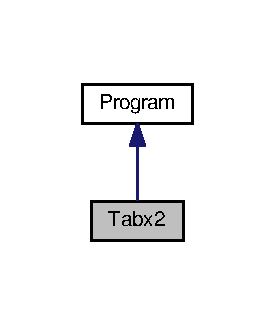
\includegraphics[width=132pt]{class_tabx2__inherit__graph}
\end{center}
\end{figure}


Diagram współpracy dla Tabx2\-:\nopagebreak
\begin{figure}[H]
\begin{center}
\leavevmode
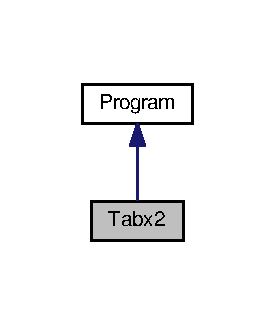
\includegraphics[width=132pt]{class_tabx2__coll__graph}
\end{center}
\end{figure}
\subsection*{Metody publiczne}
\begin{DoxyCompactItemize}
\item 
virtual bool \hyperlink{class_tabx2_a30db6636cba36a354443ec5f101fd188}{wykonaj\-\_\-program} ()
\begin{DoxyCompactList}\small\item\em Metoda wirtualna wykonaj\-\_\-program. \end{DoxyCompactList}\end{DoxyCompactItemize}
\subsection*{Dodatkowe Dziedziczone Składowe}


\subsection{Opis szczegółowy}


Definicja w linii 18 pliku tabx2.\-hh.



\subsection{Dokumentacja funkcji składowych}
\hypertarget{class_tabx2_a30db6636cba36a354443ec5f101fd188}{\index{Tabx2@{Tabx2}!wykonaj\-\_\-program@{wykonaj\-\_\-program}}
\index{wykonaj\-\_\-program@{wykonaj\-\_\-program}!Tabx2@{Tabx2}}
\subsubsection[{wykonaj\-\_\-program}]{\setlength{\rightskip}{0pt plus 5cm}bool Tabx2\-::wykonaj\-\_\-program (
\begin{DoxyParamCaption}
{}
\end{DoxyParamCaption}
)\hspace{0.3cm}{\ttfamily [virtual]}}}\label{class_tabx2_a30db6636cba36a354443ec5f101fd188}
Dokonuje przemnozenia przez 2 wszystkich danych znajdujacych sie w tablicy wskazywanej przez tab.


\begin{DoxyRetVals}{Zwracane wartości}
{\em T\-R\-U\-E} & Poprawnie dokonano mnozenia wszystkich liczb \\
\hline
{\em F\-A\-L\-S\-E} & Rozmiar tablicy danych wynosi 0 \\
\hline
\end{DoxyRetVals}


Reimplementowana z \hyperlink{class_program_ac396401ba5cade863d0e6acb727bec4e}{Program}.



Definicja w linii 6 pliku tabx2.\-cpp.



Dokumentacja dla tej klasy została wygenerowana z plików\-:\begin{DoxyCompactItemize}
\item 
\hyperlink{tabx2_8hh}{tabx2.\-hh}\item 
\hyperlink{tabx2_8cpp}{tabx2.\-cpp}\end{DoxyCompactItemize}

\chapter{Dokumentacja plików}
\input{assoctab_8hh}
\input{assoctab_8hh_source}
\hypertarget{benchmark_8cpp}{\section{Dokumentacja pliku benchmark.\-cpp}
\label{benchmark_8cpp}\index{benchmark.\-cpp@{benchmark.\-cpp}}
}


Plik zawiera metody klasy \hyperlink{class_benchmark}{Benchmark}.  


{\ttfamily \#include \char`\"{}benchmark.\-hh\char`\"{}}\\*
Wykres zależności załączania dla benchmark.\-cpp\-:\nopagebreak
\begin{figure}[H]
\begin{center}
\leavevmode
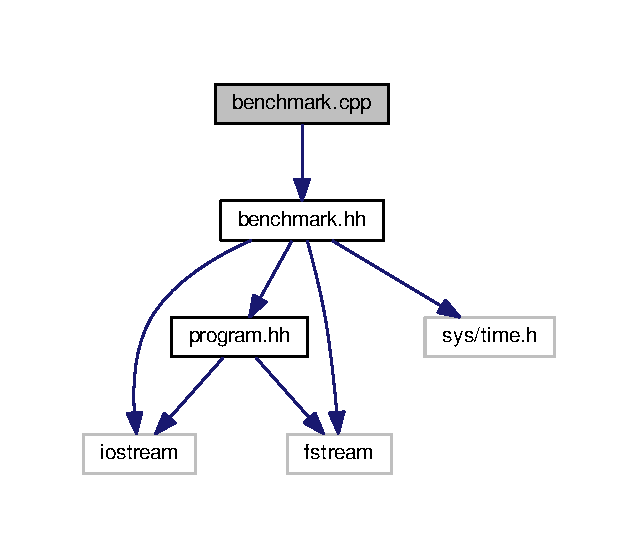
\includegraphics[width=306pt]{benchmark_8cpp__incl}
\end{center}
\end{figure}

\hypertarget{benchmark_8cpp}{\section{benchmark.\-cpp}
\label{benchmark_8cpp}\index{benchmark.\-cpp@{benchmark.\-cpp}}
}

\begin{DoxyCode}
00001 \textcolor{preprocessor}{#include "\hyperlink{benchmark_8hh}{Benchmark/benchmark.hh}"}
00002 \textcolor{preprocessor}{#include <cstdlib>}
00003 \textcolor{preprocessor}{#include <iostream>}
\hypertarget{benchmark_8cpp_source_l00008}{}\hyperlink{class_benchmark_a408a44a1d64e45b647ef6dbba2f2c3d3}{00008} \textcolor{keywordtype}{void} \hyperlink{class_benchmark_a408a44a1d64e45b647ef6dbba2f2c3d3}{Benchmark::notify}()\{
00009   \textcolor{keywordflow}{for}(\textcolor{keywordtype}{unsigned} \textcolor{keywordtype}{int} i=0; i<\hyperlink{class_subject_ad8f878ad28617e54691c4f74cd84cbe0}{obss}.\hyperlink{class_stack_a0d5ba9f716bd2c43a07cc638b8ee166f}{size}();i++)
00010     \hyperlink{class_subject_ad8f878ad28617e54691c4f74cd84cbe0}{obss}[i]->update(\hyperlink{class_benchmark_a1d0eaa6febe9b7a7f5f5147e83f60910}{amount}, \hyperlink{class_benchmark_aa88092b6164ad7d1243162d3012f729a}{mean});
00011 \}
00012 
\hypertarget{benchmark_8cpp_source_l00013}{}\hyperlink{class_benchmark_ab65889d4c2df3eb503048ab1cc6e7413}{00013} \textcolor{keywordtype}{void} \hyperlink{class_benchmark_ab65889d4c2df3eb503048ab1cc6e7413}{Benchmark::stop\_Ctimer}()\{
00014   \hyperlink{class_timer_ac05cde2d44f1a1fc40554bf78a65fe0e}{stop\_timer}();
00015   \hyperlink{class_benchmark_a7130c0718e3a3ab2fea70285dab122a2}{total}+=\hyperlink{class_timer_ab07af01194380dc8df3f3791f9aa803a}{atime};
00016   \hyperlink{class_benchmark_a3a56c7dad0b21e490f3024d5d0027f31}{counter}++;
00017 \}
00018 
\hypertarget{benchmark_8cpp_source_l00019}{}\hyperlink{class_benchmark_ac4d5360d2850510913efe07cf957f4c1}{00019} \textcolor{keywordtype}{void} \hyperlink{class_benchmark_ac4d5360d2850510913efe07cf957f4c1}{Benchmark::calc\_mean}()\{
00020   \hyperlink{class_benchmark_aa88092b6164ad7d1243162d3012f729a}{mean}=\hyperlink{class_benchmark_a7130c0718e3a3ab2fea70285dab122a2}{total}/\hyperlink{class_benchmark_a3a56c7dad0b21e490f3024d5d0027f31}{counter};
00021   std::cout << \hyperlink{class_benchmark_aa88092b6164ad7d1243162d3012f729a}{mean} << \textcolor{stringliteral}{"  "} << \hyperlink{class_benchmark_a1d0eaa6febe9b7a7f5f5147e83f60910}{amount} << \textcolor{stringliteral}{"    "} << std::endl;
00022   \hyperlink{class_benchmark_a408a44a1d64e45b647ef6dbba2f2c3d3}{notify}();
00023 \}
00024 
00025 \textcolor{keyword}{template}<\textcolor{keyword}{typename} type>
\hypertarget{benchmark_8cpp_source_l00026}{}\hyperlink{class_benchmark_ad5d8a563d9b9163758ae04d064cc38cb}{00026} \textcolor{keywordtype}{void} \hyperlink{class_benchmark_ad5d8a563d9b9163758ae04d064cc38cb}{Benchmark::runBenchmarkSort}(\textcolor{keywordtype}{void} (*f)(
      \hyperlink{class_iterable}{Iterable<type>}&, \textcolor{keywordtype}{int}, \textcolor{keywordtype}{int}), \hyperlink{class_iterable}{Iterable<type>} &container, \textcolor{keywordtype}{int} dataCount, \textcolor{keywordtype}{int} 
      repeats)\{
00027   \hyperlink{class_benchmark_a1d0eaa6febe9b7a7f5f5147e83f60910}{amount} = dataCount;
00028   \hyperlink{class_benchmark_a7130c0718e3a3ab2fea70285dab122a2}{total}=0; 
00029   \hyperlink{class_benchmark_aa88092b6164ad7d1243162d3012f729a}{mean}=0;
00030   \hyperlink{class_benchmark_a3a56c7dad0b21e490f3024d5d0027f31}{counter}=0;
00031   \textcolor{keywordflow}{for}(\textcolor{keywordtype}{int} i=1; i<=repeats; i++)\{
00032     \hyperlink{class_timer_a83d4b873e3275a61004b5679672045c0}{start\_timer}();
00033     (*f)(container, 0, \hyperlink{class_benchmark_a1d0eaa6febe9b7a7f5f5147e83f60910}{amount}-1);
00034     \hyperlink{class_benchmark_ab65889d4c2df3eb503048ab1cc6e7413}{stop\_Ctimer}();
00035   \}
00036   \hyperlink{class_benchmark_ac4d5360d2850510913efe07cf957f4c1}{calc\_mean}();
00037 \}
00038 
\hypertarget{benchmark_8cpp_source_l00039}{}\hyperlink{class_benchmark_ae9e23e7f4cf294fad57f5c98298bf874}{00039} \textcolor{keywordtype}{void} \hyperlink{class_benchmark_ae9e23e7f4cf294fad57f5c98298bf874}{Benchmark::runBenchmarkSearchGraph}(\textcolor{keywordtype}{void} (
      \hyperlink{class_graph}{Graph}::*f)(), \hyperlink{class_graph}{Graph} graph, \textcolor{keywordtype}{int} dataCount, \textcolor{keywordtype}{int} repeats)\{
00040   \hyperlink{class_benchmark_a1d0eaa6febe9b7a7f5f5147e83f60910}{amount} = dataCount;
00041   \hyperlink{class_benchmark_a7130c0718e3a3ab2fea70285dab122a2}{total}=0; 
00042   \hyperlink{class_benchmark_aa88092b6164ad7d1243162d3012f729a}{mean}=0;
00043   \hyperlink{class_benchmark_a3a56c7dad0b21e490f3024d5d0027f31}{counter}=0;
00044 
00045   \textcolor{comment}{/* DANE - spojny losowy (*/}
00046   \textcolor{keywordflow}{if}(dataCount>1)
00047     graph.\hyperlink{class_graph_a98e8eaa5f6a140aefc67a9bf07023c27}{insertE}(0, 1);
00048   \textcolor{keywordflow}{for}(\textcolor{keywordtype}{int} j=1; j<dataCount; j++)
00049     graph.\hyperlink{class_graph_a98e8eaa5f6a140aefc67a9bf07023c27}{insertE}(j, rand()%j);
00050   \textcolor{comment}{/* DANE - 0 ze wszystkimi }
00051 \textcolor{comment}{     for(int j=0; j<dataCount; j++)}
00052 \textcolor{comment}{     graph.insertE(0,j);*/}
00053   \textcolor{comment}{/* DANE - LISTA }
00054 \textcolor{comment}{     for(int j=0; j<=dataCount-2; j++)\{}
00055 \textcolor{comment}{     graph.insertE(j, j+1);}
00056 \textcolor{comment}{     \}*/}
00057   \textcolor{keywordflow}{for}(\textcolor{keywordtype}{int} i=1; i<=repeats; i++)\{
00058     \hyperlink{class_timer_a83d4b873e3275a61004b5679672045c0}{start\_timer}();
00059     (graph.*f)();
00060     \hyperlink{class_benchmark_ab65889d4c2df3eb503048ab1cc6e7413}{stop\_Ctimer}();
00061   \}
00062   \hyperlink{class_benchmark_ac4d5360d2850510913efe07cf957f4c1}{calc\_mean}();
00063 \}
00064 
00065 
00066 
\end{DoxyCode}

\hypertarget{benchmark_8hh}{\section{Dokumentacja pliku benchmark.\-hh}
\label{benchmark_8hh}\index{benchmark.\-hh@{benchmark.\-hh}}
}


Definicja klasy \hyperlink{class_benchmark}{Benchmark}.  


{\ttfamily \#include $<$iostream$>$}\\*
{\ttfamily \#include \char`\"{}program.\-hh\char`\"{}}\\*
{\ttfamily \#include $<$sys/time.\-h$>$}\\*
{\ttfamily \#include $<$fstream$>$}\\*
Wykres zależności załączania dla benchmark.\-hh\-:
\nopagebreak
\begin{figure}[H]
\begin{center}
\leavevmode
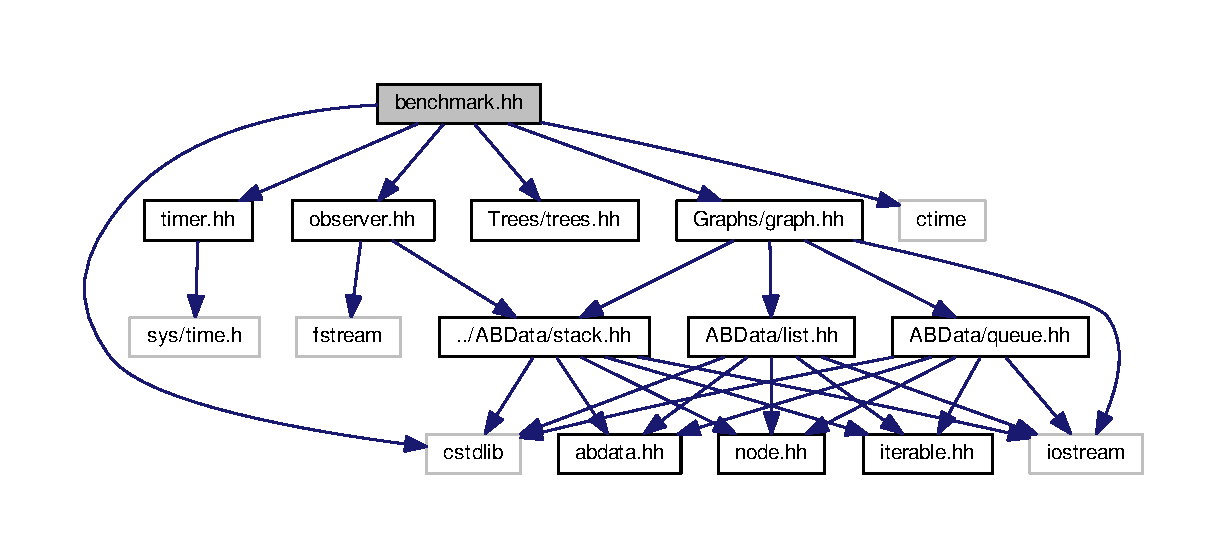
\includegraphics[width=306pt]{benchmark_8hh__incl}
\end{center}
\end{figure}
Ten wykres pokazuje, które pliki bezpośrednio lub pośrednio załączają ten plik\-:\nopagebreak
\begin{figure}[H]
\begin{center}
\leavevmode
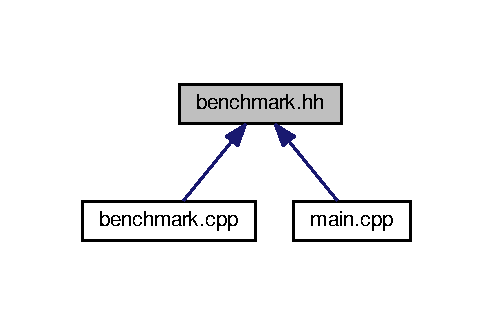
\includegraphics[width=237pt]{benchmark_8hh__dep__incl}
\end{center}
\end{figure}
\subsection*{Komponenty}
\begin{DoxyCompactItemize}
\item 
class \hyperlink{class_benchmark}{Benchmark}
\begin{DoxyCompactList}\small\item\em Klasa \hyperlink{class_benchmark}{Benchmark}. \end{DoxyCompactList}\end{DoxyCompactItemize}

\hypertarget{benchmark_8hh}{\section{benchmark.\-hh}
\label{benchmark_8hh}\index{benchmark.\-hh@{benchmark.\-hh}}
}

\begin{DoxyCode}
00001 \textcolor{comment}{//benchmark.hh}
00002 
00003 \textcolor{preprocessor}{#ifndef BENCHMARK\_HH}
00004 \textcolor{preprocessor}{}\textcolor{preprocessor}{#define BENCHMARK\_HH}
00005 \textcolor{preprocessor}{}
00006 \textcolor{preprocessor}{#include <iostream>}
00007 \textcolor{preprocessor}{#include "\hyperlink{program_8hh}{program.hh}"}
00008 \textcolor{preprocessor}{#include <sys/time.h>}
00009 \textcolor{preprocessor}{#include <fstream>}
00010 
00016 \textcolor{keyword}{using namespace }std;
00017 
\hypertarget{benchmark_8hh_source_l00023}{}\hyperlink{class_benchmark}{00023} \textcolor{keyword}{class }\hyperlink{class_benchmark}{Benchmark}\{
00024 \textcolor{keyword}{private}:
\hypertarget{benchmark_8hh_source_l00030}{}\hyperlink{class_benchmark_a2b145dd2458fea33d6df41f310058bec}{00030}   timeval t1, \hyperlink{class_benchmark_a2b145dd2458fea33d6df41f310058bec}{t2};
00031 
\hypertarget{benchmark_8hh_source_l00037}{}\hyperlink{class_benchmark_ab72b3cbe324970fd8c738f03718d52fc}{00037}   \textcolor{keywordtype}{double} \hyperlink{class_benchmark_ab72b3cbe324970fd8c738f03718d52fc}{czas\_pomiaru};
00038 
00039 \textcolor{keyword}{public}:
00045   \textcolor{keywordtype}{void} rozpocznij\_pomiar();
00046 
00052   \textcolor{keywordtype}{void} zakoncz\_pomiar();
00053 
00066   \textcolor{keywordtype}{double} testuj(\hyperlink{class_program}{Program} &program,\textcolor{keywordtype}{char}* dane, \textcolor{keywordtype}{int} ilosc\_danych, \textcolor{keywordtype}{int} ilosc\_testow);
00067 
00081   \textcolor{keywordtype}{double} testuj\_strukture(\hyperlink{class_program}{Program} &program,\textcolor{keywordtype}{char}* dane, \textcolor{keywordtype}{int} ilosc\_danych, \textcolor{keywordtype}{int} ilosc\_testow);
00082 \};
00083 
00084 \textcolor{preprocessor}{#endif}
\end{DoxyCode}

\input{hashtab_8cpp}
\input{hashtab_8cpp_source}
\hypertarget{lista_8hh}{\section{Dokumentacja pliku lista.\-hh}
\label{lista_8hh}\index{lista.\-hh@{lista.\-hh}}
}


Definicja klasy \hyperlink{class_lista}{Lista}.  


{\ttfamily \#include \char`\"{}program.\-hh\char`\"{}}\\*
Wykres zależności załączania dla lista.\-hh\-:\nopagebreak
\begin{figure}[H]
\begin{center}
\leavevmode
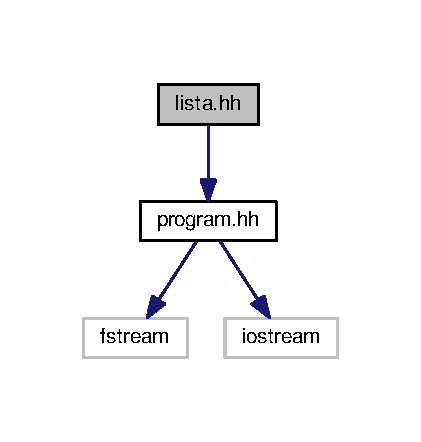
\includegraphics[width=202pt]{lista_8hh__incl}
\end{center}
\end{figure}
Ten wykres pokazuje, które pliki bezpośrednio lub pośrednio załączają ten plik\-:\nopagebreak
\begin{figure}[H]
\begin{center}
\leavevmode
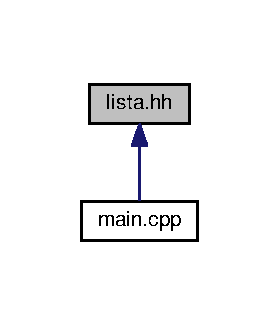
\includegraphics[width=134pt]{lista_8hh__dep__incl}
\end{center}
\end{figure}
\subsection*{Komponenty}
\begin{DoxyCompactItemize}
\item 
class \hyperlink{class_lista}{Lista$<$ type, type2 $>$}
\item 
struct \hyperlink{struct_lista_1_1pole}{Lista$<$ type, type2 $>$\-::pole}
\begin{DoxyCompactList}\small\item\em Struktura pole. \end{DoxyCompactList}\end{DoxyCompactItemize}

\hypertarget{lista_8hh}{\section{lista.\-hh}
\label{lista_8hh}\index{lista.\-hh@{lista.\-hh}}
}

\begin{DoxyCode}
00001 \textcolor{comment}{//lista.hh}
00002 \textcolor{preprocessor}{#ifndef LISTA\_HH}
00003 \textcolor{preprocessor}{}\textcolor{preprocessor}{#define LISTA\_HH}
00004 \textcolor{preprocessor}{}
00005 \textcolor{preprocessor}{#include "\hyperlink{program_8hh}{program.hh}"}
00006 
\hypertarget{lista_8hh_source_l00019}{}\hyperlink{structpole}{00019} \textcolor{keyword}{struct }\hyperlink{structpole}{pole}\{
\hypertarget{lista_8hh_source_l00020}{}\hyperlink{structpole_a22b23161f03ecb022f751026360b8348}{00020}   \textcolor{keywordtype}{int} \hyperlink{structpole_a22b23161f03ecb022f751026360b8348}{wartosc};
\hypertarget{lista_8hh_source_l00021}{}\hyperlink{structpole_a323a379be6456423a7d002d2f67a7a23}{00021}   \hyperlink{structpole}{pole} *\hyperlink{structpole_a323a379be6456423a7d002d2f67a7a23}{next};
\hypertarget{lista_8hh_source_l00022}{}\hyperlink{structpole_a6d02cdb7a21cebb2c0a3c5c9936dd038}{00022}   \hyperlink{structpole_a6d02cdb7a21cebb2c0a3c5c9936dd038}{pole}()\{\hyperlink{structpole_a22b23161f03ecb022f751026360b8348}{wartosc}=0; \hyperlink{structpole_a323a379be6456423a7d002d2f67a7a23}{next}=NULL;\}
00023 \};
00024 
\hypertarget{lista_8hh_source_l00025}{}\hyperlink{class_lista}{00025} \textcolor{keyword}{class }\hyperlink{class_lista}{Lista}: \textcolor{keyword}{public} \hyperlink{class_program}{Program}\{
\hypertarget{lista_8hh_source_l00026}{}\hyperlink{class_lista_ae9ddc4b39562b5382a9c2559f2e4b421}{00026}   \hyperlink{structpole}{pole} *\hyperlink{class_lista_ae9ddc4b39562b5382a9c2559f2e4b421}{first};
00027 \textcolor{keyword}{public}:
\hypertarget{lista_8hh_source_l00033}{}\hyperlink{class_lista_a1f668b36909182ef1360b48503529a31}{00033}  \hyperlink{class_lista_a1f668b36909182ef1360b48503529a31}{Lista}()\{
00034     \hyperlink{class_lista_ae9ddc4b39562b5382a9c2559f2e4b421}{first} = NULL;
00035   \}
00043   \textcolor{keywordtype}{void} \hyperlink{class_lista_ac844f54fca7aaadf53620d1e147068e3}{push}(\textcolor{keywordtype}{int} x);
00049   \textcolor{keywordtype}{void} \hyperlink{class_lista_a5bece8ad206f5e6497f8cc23419ed051}{pop}();
00057   \textcolor{keywordtype}{int} \hyperlink{class_lista_a3836382e3cf53b6ea281937d045d181c}{size}();
00058 
00068   \textcolor{keywordtype}{bool} \hyperlink{class_program_ac396401ba5cade863d0e6acb727bec4e}{wykonaj\_program}(\textcolor{keywordtype}{char}* nazwa\_pliku,\textcolor{keywordtype}{int} ilosc\_danych);
00069 
00077   \textcolor{keywordtype}{void} \hyperlink{class_lista_af73c0c1eba31c0d82d107d57e99fc3d7}{wyczysc\_dane}(\textcolor{keywordtype}{int} ile);
00078 \};
00079 
00080 \textcolor{preprocessor}{#endif}
\end{DoxyCode}

\hypertarget{lista__tab_8cpp}{\section{Dokumentacja pliku lista\-\_\-tab.\-cpp}
\label{lista__tab_8cpp}\index{lista\-\_\-tab.\-cpp@{lista\-\_\-tab.\-cpp}}
}


Zawiera definicje metod klasy \hyperlink{class_lista}{Lista}.  


{\ttfamily \#include \char`\"{}lista\-\_\-tab.\-hh\char`\"{}}\\*
Wykres zależności załączania dla lista\-\_\-tab.\-cpp\-:\nopagebreak
\begin{figure}[H]
\begin{center}
\leavevmode
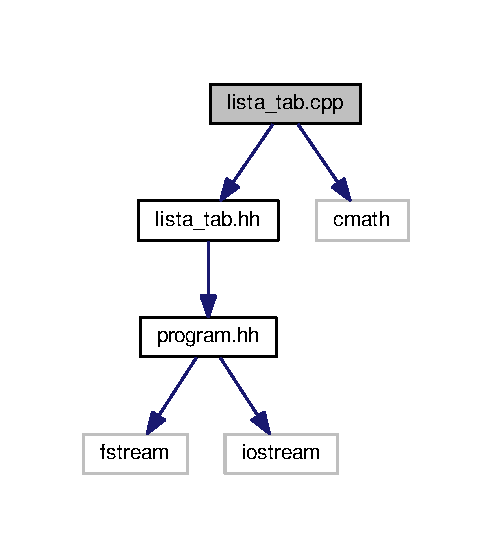
\includegraphics[width=202pt]{lista__tab_8cpp__incl}
\end{center}
\end{figure}

\hypertarget{lista__tab_8cpp}{\section{lista\-\_\-tab.\-cpp}
\label{lista__tab_8cpp}\index{lista\-\_\-tab.\-cpp@{lista\-\_\-tab.\-cpp}}
}

\begin{DoxyCode}
00001 \textcolor{comment}{//lista\_tab.cpp}
00002 \textcolor{preprocessor}{#include "\hyperlink{lista__tab_8hh}{lista\_tab.hh}"}
00003 \textcolor{preprocessor}{#include <cmath>}
00004 
00008 \textcolor{comment}{// ZWIEKSZA SIE O 1}
00009 \textcolor{comment}{/*void Lista\_tab::push(int x)\{}
00010 \textcolor{comment}{  if(rozmiar==0)\{}
00011 \textcolor{comment}{    tab = new int [1];}
00012 \textcolor{comment}{    rozmiar=1;}
00013 \textcolor{comment}{    iterator=0;}
00014 \textcolor{comment}{    tab[iterator]=x;}
00015 \textcolor{comment}{  \}}
00016 \textcolor{comment}{  else\{}
00017 \textcolor{comment}{    if(iterator<rozmiar-1)\{}
00018 \textcolor{comment}{      tab[++iterator]=x;}
00019 \textcolor{comment}{    \}}
00020 \textcolor{comment}{    else if(iterator>=rozmiar-1)\{}
00021 \textcolor{comment}{      int *tmp = new int[rozmiar+1];}
00022 \textcolor{comment}{      for(int i=0;i<=iterator;i++)}
00023 \textcolor{comment}{    tmp[i] = tab[i];}
00024 \textcolor{comment}{      delete [] tab;}
00025 \textcolor{comment}{      tab = tmp;}
00026 \textcolor{comment}{      tab[++iterator]=x;}
00027 \textcolor{comment}{      rozmiar++;}
00028 \textcolor{comment}{    \}}
00029 \textcolor{comment}{  \}}
00030 \textcolor{comment}{  \}*/}
00031 \textcolor{comment}{//TABLICA POWIEKSZANA DWUKROTNIE}
\hypertarget{lista__tab_8cpp_source_l00032}{}\hyperlink{lista__tab_8cpp_a536abf9d26ff06b830492601f58eb288}{00032} \textcolor{keywordtype}{void} \hyperlink{lista__tab_8cpp_a536abf9d26ff06b830492601f58eb288}{zamien}(\textcolor{keywordtype}{int} *wsk, \textcolor{keywordtype}{int} i, \textcolor{keywordtype}{int} j)\{
00033   \textcolor{keywordtype}{int} tmp;
00034   tmp=wsk[i];
00035   wsk[i]=wsk[j];
00036   wsk[j]=tmp;
00037 \}
00038 
\hypertarget{lista__tab_8cpp_source_l00039}{}\hyperlink{class_lista__tab_a800998768639b41b5be5c52ec4ccbda4}{00039} \textcolor{keywordtype}{void} \hyperlink{class_lista__tab_a800998768639b41b5be5c52ec4ccbda4}{Lista\_tab::push}(\textcolor{keywordtype}{int} x)\{
00040   \textcolor{keywordflow}{if}(\hyperlink{class_lista__tab_a59e0425d896070457d1f3456b91842fd}{rozmiar}==0)\{
00041     \hyperlink{class_lista__tab_a123dfb670e5a5592e512c41cc4faf14e}{tab} = \textcolor{keyword}{new} \textcolor{keywordtype}{int} [1];
00042     \hyperlink{class_lista__tab_a59e0425d896070457d1f3456b91842fd}{rozmiar}=1;
00043     \hyperlink{class_lista__tab_afd2c6ba3ae15e658890641b188c7ed39}{iterator}=0;
00044     \hyperlink{class_lista__tab_a123dfb670e5a5592e512c41cc4faf14e}{tab}[\hyperlink{class_lista__tab_afd2c6ba3ae15e658890641b188c7ed39}{iterator}]=x;
00045   \}
00046   \textcolor{keywordflow}{else}\{
00047     \textcolor{keywordflow}{if}(\hyperlink{class_lista__tab_afd2c6ba3ae15e658890641b188c7ed39}{iterator}<\hyperlink{class_lista__tab_a59e0425d896070457d1f3456b91842fd}{rozmiar}-1)\{
00048       \hyperlink{class_lista__tab_a123dfb670e5a5592e512c41cc4faf14e}{tab}[++\hyperlink{class_lista__tab_afd2c6ba3ae15e658890641b188c7ed39}{iterator}]=x;
00049     \}
00050     \textcolor{keywordflow}{else} \textcolor{keywordflow}{if}(\hyperlink{class_lista__tab_afd2c6ba3ae15e658890641b188c7ed39}{iterator}>=\hyperlink{class_lista__tab_a59e0425d896070457d1f3456b91842fd}{rozmiar}-1)\{
00051       \textcolor{keywordtype}{int} *tmp = \textcolor{keyword}{new} \textcolor{keywordtype}{int}[2*\hyperlink{class_lista__tab_a59e0425d896070457d1f3456b91842fd}{rozmiar}];
00052       \textcolor{keywordflow}{for}(\textcolor{keywordtype}{int} i=0;i<=\hyperlink{class_lista__tab_afd2c6ba3ae15e658890641b188c7ed39}{iterator};i++)
00053     tmp[i] = \hyperlink{class_lista__tab_a123dfb670e5a5592e512c41cc4faf14e}{tab}[i];
00054       \textcolor{keyword}{delete} [] \hyperlink{class_lista__tab_a123dfb670e5a5592e512c41cc4faf14e}{tab};
00055       \hyperlink{class_lista__tab_a123dfb670e5a5592e512c41cc4faf14e}{tab} = tmp;
00056       \hyperlink{class_lista__tab_a123dfb670e5a5592e512c41cc4faf14e}{tab}[++\hyperlink{class_lista__tab_afd2c6ba3ae15e658890641b188c7ed39}{iterator}]=x;
00057       \hyperlink{class_lista__tab_a59e0425d896070457d1f3456b91842fd}{rozmiar}*=2;
00058     \}
00059   \}
00060 \}
00061 
00062 
\hypertarget{lista__tab_8cpp_source_l00063}{}\hyperlink{class_lista__tab_affc42a7ffc6eda21076fc56eae38e980}{00063} \textcolor{keywordtype}{void} \hyperlink{class_lista__tab_affc42a7ffc6eda21076fc56eae38e980}{Lista\_tab::pop}()\{
00064   \textcolor{keywordflow}{if}(\hyperlink{class_lista__tab_a59e0425d896070457d1f3456b91842fd}{rozmiar} == 0)\{
00065     cerr<<\textcolor{stringliteral}{"Lista jest pusta!"}<<endl;
00066   \}
00067   \hyperlink{class_lista__tab_afd2c6ba3ae15e658890641b188c7ed39}{iterator}--;
00068   \textcolor{keywordflow}{if}(\hyperlink{class_lista__tab_afd2c6ba3ae15e658890641b188c7ed39}{iterator}<0.25*(\hyperlink{class_lista__tab_a59e0425d896070457d1f3456b91842fd}{rozmiar}-1))\{
00069     \textcolor{keywordtype}{int} *tmp = \textcolor{keyword}{new} \textcolor{keywordtype}{int}[\hyperlink{class_lista__tab_afd2c6ba3ae15e658890641b188c7ed39}{iterator}+1];
00070     \textcolor{keywordflow}{for}(\textcolor{keywordtype}{int} i=0;i<=\hyperlink{class_lista__tab_afd2c6ba3ae15e658890641b188c7ed39}{iterator};i++)\{
00071       tmp[i]=\hyperlink{class_lista__tab_a123dfb670e5a5592e512c41cc4faf14e}{tab}[i];
00072     \}  
00073     \textcolor{keyword}{delete} [] \hyperlink{class_lista__tab_a123dfb670e5a5592e512c41cc4faf14e}{tab};
00074     \hyperlink{class_lista__tab_a123dfb670e5a5592e512c41cc4faf14e}{tab} = tmp;
00075     \hyperlink{class_lista__tab_a59e0425d896070457d1f3456b91842fd}{rozmiar} = \hyperlink{class_lista__tab_afd2c6ba3ae15e658890641b188c7ed39}{iterator}+1;
00076   \}
00077 \}
00078 
00079 
\hypertarget{lista__tab_8cpp_source_l00080}{}\hyperlink{class_lista__tab_af092dd7943f7cd5ff407485f2991a1e4}{00080} \textcolor{keywordtype}{int} \hyperlink{class_lista__tab_af092dd7943f7cd5ff407485f2991a1e4}{Lista\_tab::size}()\{
00081   \textcolor{keywordflow}{return} \hyperlink{class_lista__tab_afd2c6ba3ae15e658890641b188c7ed39}{iterator}+1;
00082 \}
00083 
\hypertarget{lista__tab_8cpp_source_l00084}{}\hyperlink{class_lista__tab_ac9adc6ecc7348c5e1871b239c1313405}{00084} \textcolor{keywordtype}{bool} \hyperlink{class_program_ac396401ba5cade863d0e6acb727bec4e}{Lista\_tab::wykonaj\_program}(\textcolor{keywordtype}{char}* nazwa\_pliku, \textcolor{keywordtype}{int} ilosc\_danych)\{
00085   \textcolor{keywordtype}{int} tmp;
00086   \hyperlink{class_program_aac2f72538e24e533c327fe5546a59210}{plik\_we}.open(nazwa\_pliku);
00087   \textcolor{keywordflow}{if}(\hyperlink{class_program_aac2f72538e24e533c327fe5546a59210}{plik\_we}.good()==\textcolor{keyword}{false})\{
00088     cerr<<\textcolor{stringliteral}{"Blad odczytu pliku!"}<<endl;
00089     \textcolor{keywordflow}{return} \textcolor{keyword}{false};
00090   \}
00091   \hyperlink{class_program_aac2f72538e24e533c327fe5546a59210}{plik\_we} >> \hyperlink{class_program_a3b5a10104019b9daa23ce4a5f5533820}{rozmiar\_tab};  \textcolor{comment}{//pozbyc sie pierwszej liczby z pliku z danymi}
00092   \textcolor{keywordflow}{for}(\textcolor{keywordtype}{int} i=0;i<ilosc\_danych;i++)\{
00093     \hyperlink{class_program_aac2f72538e24e533c327fe5546a59210}{plik\_we} >> tmp;
00094     \hyperlink{class_lista__tab_a800998768639b41b5be5c52ec4ccbda4}{push}(tmp);
00095   \}
00096   \hyperlink{class_program_aac2f72538e24e533c327fe5546a59210}{plik\_we}.close();
00097   \textcolor{keywordflow}{return} \textcolor{keyword}{true};
00098 \}
00099 
\hypertarget{lista__tab_8cpp_source_l00100}{}\hyperlink{class_lista__tab_a506a6de79a600bac8316a6caf9878528}{00100} \textcolor{keywordtype}{void} \hyperlink{class_lista__tab_a506a6de79a600bac8316a6caf9878528}{Lista\_tab::wyczysc\_dane}(\textcolor{keywordtype}{int} ile)\{
00101   \textcolor{keyword}{delete} [] \hyperlink{class_lista__tab_a123dfb670e5a5592e512c41cc4faf14e}{tab};
00102   \hyperlink{class_lista__tab_a59e0425d896070457d1f3456b91842fd}{rozmiar} = 0;
00103   \hyperlink{class_lista__tab_afd2c6ba3ae15e658890641b188c7ed39}{iterator} = 0;
00104   \hyperlink{class_lista__tab_a123dfb670e5a5592e512c41cc4faf14e}{tab} = NULL;
00105 \}
00106 
\hypertarget{lista__tab_8cpp_source_l00107}{}\hyperlink{class_lista__tab_a409e9a4edbef4337980c7184b6cbfb63}{00107} \textcolor{keywordtype}{void} \hyperlink{class_lista__tab_a409e9a4edbef4337980c7184b6cbfb63}{Lista\_tab::mergesort}(\textcolor{keywordtype}{int} beg, \textcolor{keywordtype}{int} end)\{
00108   \textcolor{keywordtype}{int} tmp[end+1];
00109   \textcolor{keywordtype}{int} mid = (beg+end+1)/2; \textcolor{keywordtype}{int} i1, i2,i;
00110   \textcolor{keywordflow}{if}(mid-beg>1)
00111     \hyperlink{class_lista__tab_a409e9a4edbef4337980c7184b6cbfb63}{mergesort}(beg,mid-1);
00112   \textcolor{keywordflow}{if}(end-mid>0)
00113     \hyperlink{class_lista__tab_a409e9a4edbef4337980c7184b6cbfb63}{mergesort}(mid,end);
00114   i1=beg; i2=mid;
00115   \textcolor{keywordflow}{for}(i=beg; i<=end; i++)
00116     tmp[i]=((i1==mid)||((i2<=end)&&(\hyperlink{class_lista__tab_a123dfb670e5a5592e512c41cc4faf14e}{tab}[i1] > \hyperlink{class_lista__tab_a123dfb670e5a5592e512c41cc4faf14e}{tab}[i2]))) ? \hyperlink{class_lista__tab_a123dfb670e5a5592e512c41cc4faf14e}{tab}[i2++] : 
      \hyperlink{class_lista__tab_a123dfb670e5a5592e512c41cc4faf14e}{tab}[i1++];
00117   \textcolor{keywordflow}{for}(i=beg; i<=end; i++) \hyperlink{class_lista__tab_a123dfb670e5a5592e512c41cc4faf14e}{tab}[i]=tmp[i];
00118 \}
00119 
\hypertarget{lista__tab_8cpp_source_l00120}{}\hyperlink{class_lista__tab_ac9dc3e6ccaff0aef1a1370c1a83c48d9}{00120} \textcolor{keywordtype}{void} \hyperlink{class_lista__tab_ac9dc3e6ccaff0aef1a1370c1a83c48d9}{Lista\_tab::heapsort}()\{
00121 
00122   \textcolor{keywordflow}{if}(\hyperlink{class_lista__tab_af092dd7943f7cd5ff407485f2991a1e4}{size}()>1)\{
00123 
00124     \textcolor{keywordtype}{int} root, swap, child, val, start,end;
00125 
00126     \textcolor{comment}{//heapify}
00127     start=(\hyperlink{class_lista__tab_af092dd7943f7cd5ff407485f2991a1e4}{size}()-2)/2;
00128     \textcolor{keywordflow}{while}(start>=0)\{
00129       \textcolor{comment}{//siftdown}
00130       root = start; end = \hyperlink{class_lista__tab_af092dd7943f7cd5ff407485f2991a1e4}{size}()-1;
00131       \textcolor{keywordflow}{while}(((root*2)+1)<=end)\{
00132     child = (root*2)+1; \textcolor{comment}{//left child}
00133     swap = root;      \textcolor{comment}{//remembers child}
00134     \textcolor{keywordflow}{if}(\hyperlink{class_lista__tab_a123dfb670e5a5592e512c41cc4faf14e}{tab}[swap]<\hyperlink{class_lista__tab_a123dfb670e5a5592e512c41cc4faf14e}{tab}[child])
00135       swap = child;
00136     \textcolor{keywordflow}{if}(((child+1)<=end) && (\hyperlink{class_lista__tab_a123dfb670e5a5592e512c41cc4faf14e}{tab}[swap]<\hyperlink{class_lista__tab_a123dfb670e5a5592e512c41cc4faf14e}{tab}[child+1]))
00137       swap = child+1;
00138     \textcolor{keywordflow}{if}(swap==root) \textcolor{keywordflow}{break};
00139     \textcolor{keywordflow}{else}\{
00140       val=\hyperlink{class_lista__tab_a123dfb670e5a5592e512c41cc4faf14e}{tab}[root];
00141       \hyperlink{class_lista__tab_a123dfb670e5a5592e512c41cc4faf14e}{tab}[root]=\hyperlink{class_lista__tab_a123dfb670e5a5592e512c41cc4faf14e}{tab}[swap];
00142       \hyperlink{class_lista__tab_a123dfb670e5a5592e512c41cc4faf14e}{tab}[swap]=val;
00143       root=swap;
00144     \}
00145       \}
00146       start--;
00147     \}
00148     \textcolor{comment}{//}
00149     end=\hyperlink{class_lista__tab_af092dd7943f7cd5ff407485f2991a1e4}{size}()-1;
00150     \textcolor{keywordflow}{while}(end>0)\{
00151       val=\hyperlink{class_lista__tab_a123dfb670e5a5592e512c41cc4faf14e}{tab}[end];
00152       \hyperlink{class_lista__tab_a123dfb670e5a5592e512c41cc4faf14e}{tab}[end]=\hyperlink{class_lista__tab_a123dfb670e5a5592e512c41cc4faf14e}{tab}[0];
00153       \hyperlink{class_lista__tab_a123dfb670e5a5592e512c41cc4faf14e}{tab}[0]=val;
00154       end--;
00155       \textcolor{comment}{//siftdown}
00156       root = 0; 
00157       \textcolor{keywordflow}{while}(root*2+1<=end)\{
00158     child = root*2+1; \textcolor{comment}{//left child}
00159     swap = root;      \textcolor{comment}{//remembers child}
00160 
00161     \textcolor{keywordflow}{if}(\hyperlink{class_lista__tab_a123dfb670e5a5592e512c41cc4faf14e}{tab}[swap]<\hyperlink{class_lista__tab_a123dfb670e5a5592e512c41cc4faf14e}{tab}[child])
00162       swap = child;
00163     \textcolor{keywordflow}{if}(child+1<=end && \hyperlink{class_lista__tab_a123dfb670e5a5592e512c41cc4faf14e}{tab}[swap]<\hyperlink{class_lista__tab_a123dfb670e5a5592e512c41cc4faf14e}{tab}[child+1])
00164       swap = child+1;
00165     \textcolor{keywordflow}{if}(swap==root) \textcolor{keywordflow}{break};
00166     \textcolor{keywordflow}{else}\{
00167       val=\hyperlink{class_lista__tab_a123dfb670e5a5592e512c41cc4faf14e}{tab}[root];
00168       \hyperlink{class_lista__tab_a123dfb670e5a5592e512c41cc4faf14e}{tab}[root]=\hyperlink{class_lista__tab_a123dfb670e5a5592e512c41cc4faf14e}{tab}[swap];
00169       \hyperlink{class_lista__tab_a123dfb670e5a5592e512c41cc4faf14e}{tab}[swap]=val;
00170       root=swap;
00171     \}
00172       \}
00173     \}
00174   \}
00175 \}
00176 
\hypertarget{lista__tab_8cpp_source_l00177}{}\hyperlink{class_lista__tab_a1a20726180b67b7cf2a669cafd6d3ca3}{00177} \textcolor{keywordtype}{void} \hyperlink{class_lista__tab_a1a20726180b67b7cf2a669cafd6d3ca3}{Lista\_tab::quicksort}(\textcolor{keywordtype}{int} left, \textcolor{keywordtype}{int} right)\{
00178   \textcolor{keywordtype}{int} i=(right+left)/2;
00179   \textcolor{keywordtype}{int} j=0;
00180  
00181   \textcolor{keywordflow}{if}(\hyperlink{class_lista__tab_a123dfb670e5a5592e512c41cc4faf14e}{tab}[right]<\hyperlink{class_lista__tab_a123dfb670e5a5592e512c41cc4faf14e}{tab}[left])
00182     \hyperlink{lista__tab_8cpp_a536abf9d26ff06b830492601f58eb288}{zamien}(\hyperlink{class_lista__tab_a123dfb670e5a5592e512c41cc4faf14e}{tab},left,right);
00183   \textcolor{keywordflow}{if}(\hyperlink{class_lista__tab_a123dfb670e5a5592e512c41cc4faf14e}{tab}[i] < \hyperlink{class_lista__tab_a123dfb670e5a5592e512c41cc4faf14e}{tab}[left])
00184     \hyperlink{lista__tab_8cpp_a536abf9d26ff06b830492601f58eb288}{zamien}(\hyperlink{class_lista__tab_a123dfb670e5a5592e512c41cc4faf14e}{tab},i,left);
00185   \textcolor{keywordflow}{if}(\hyperlink{class_lista__tab_a123dfb670e5a5592e512c41cc4faf14e}{tab}[right]<\hyperlink{class_lista__tab_a123dfb670e5a5592e512c41cc4faf14e}{tab}[i])
00186     \hyperlink{lista__tab_8cpp_a536abf9d26ff06b830492601f58eb288}{zamien}(\hyperlink{class_lista__tab_a123dfb670e5a5592e512c41cc4faf14e}{tab},right,i);
00187   \textcolor{keywordtype}{int} piwot=\hyperlink{class_lista__tab_a123dfb670e5a5592e512c41cc4faf14e}{tab}[i];
00188   i=left; j = right;
00189   \textcolor{keywordflow}{do}\{
00190     \textcolor{keywordflow}{while}(\hyperlink{class_lista__tab_a123dfb670e5a5592e512c41cc4faf14e}{tab}[i]<piwot) i++;
00191     \textcolor{keywordflow}{while}(\hyperlink{class_lista__tab_a123dfb670e5a5592e512c41cc4faf14e}{tab}[j]>piwot) j--;
00192     \textcolor{keywordflow}{if}(i<=j)\{
00193       \hyperlink{lista__tab_8cpp_a536abf9d26ff06b830492601f58eb288}{zamien}(\hyperlink{class_lista__tab_a123dfb670e5a5592e512c41cc4faf14e}{tab},i,j);
00194       i++; j--;
00195     \}
00196   \}\textcolor{keywordflow}{while}(i<=j);
00197   
00198   \textcolor{keywordflow}{if}(j>left)
00199     \hyperlink{class_lista__tab_a1a20726180b67b7cf2a669cafd6d3ca3}{quicksort}(left,j);
00200   \textcolor{keywordflow}{if}(i<right)
00201     \hyperlink{class_lista__tab_a1a20726180b67b7cf2a669cafd6d3ca3}{quicksort}(i,right);
00202 \}
00203 
00204 
00205 
\hypertarget{lista__tab_8cpp_source_l00206}{}\hyperlink{lista__tab_8cpp_aba1e73e8a2200c8303fa031d788bd069}{00206} \textcolor{keywordtype}{int} \hyperlink{lista__tab_8cpp_aba1e73e8a2200c8303fa031d788bd069}{quicky}(\textcolor{keywordtype}{int} *wsk, \textcolor{keywordtype}{int} left, \textcolor{keywordtype}{int} right)\{
00207   \textcolor{keywordtype}{int} i, j; 
00208   i = (left+right)/2;
00209   \textcolor{keywordflow}{if}(wsk[right]<wsk[left])
00210     \hyperlink{lista__tab_8cpp_a536abf9d26ff06b830492601f58eb288}{zamien}(wsk,left,right);
00211   \textcolor{keywordflow}{if}(wsk[i] < wsk[left])
00212     \hyperlink{lista__tab_8cpp_a536abf9d26ff06b830492601f58eb288}{zamien}(wsk,i,left);
00213   \textcolor{keywordflow}{if}(wsk[right]<wsk[i])
00214     \hyperlink{lista__tab_8cpp_a536abf9d26ff06b830492601f58eb288}{zamien}(wsk,right,i);
00215 
00216   \textcolor{keywordflow}{for} (i=left, j=right-2; ; )
00217     \{
00218       \textcolor{keywordflow}{for} ( ; wsk[i]<wsk[right-1]; ++i);
00219       \textcolor{keywordflow}{for} ( ; j>=left && wsk[j]>wsk[right-1]; --j);
00220       \textcolor{keywordflow}{if} (i<j)
00221     \hyperlink{lista__tab_8cpp_a536abf9d26ff06b830492601f58eb288}{zamien}(wsk,i++,j--);
00222       \textcolor{keywordflow}{else} \textcolor{keywordflow}{break};
00223     \}
00224   \hyperlink{lista__tab_8cpp_a536abf9d26ff06b830492601f58eb288}{zamien}(wsk,i,right-1);
00225   \textcolor{keywordflow}{return} i;
00226 \}
00227 
\hypertarget{lista__tab_8cpp_source_l00228}{}\hyperlink{lista__tab_8cpp_a1deb3e2758fa73fd8968484f96d1c982}{00228} \textcolor{keywordtype}{void} \hyperlink{lista__tab_8cpp_a1deb3e2758fa73fd8968484f96d1c982}{heapsort}(\textcolor{keywordtype}{int} *wsk, \textcolor{keywordtype}{int} rozmiar)\{
00229   \textcolor{keywordflow}{if}(rozmiar>1)\{
00230 
00231     \textcolor{keywordtype}{int} root, swap, child, val, start,end;
00232 
00233     \textcolor{comment}{//heapify}
00234     start=(rozmiar-2)/2;
00235     \textcolor{keywordflow}{while}(start>=0)\{
00236       \textcolor{comment}{//siftdown}
00237       root = start; end = rozmiar-1;
00238       \textcolor{keywordflow}{while}(((root*2)+1)<=end)\{
00239     child = (root*2)+1; \textcolor{comment}{//left child}
00240     swap = root;      \textcolor{comment}{//remembers child}
00241     \textcolor{keywordflow}{if}(wsk[swap]<wsk[child])
00242       swap = child;
00243     \textcolor{keywordflow}{if}(((child+1)<=end) && (wsk[swap]<wsk[child+1]))
00244       swap = child+1;
00245     \textcolor{keywordflow}{if}(swap==root) \textcolor{keywordflow}{break};
00246     \textcolor{keywordflow}{else}\{
00247       val=wsk[root];
00248       wsk[root]=wsk[swap];
00249       wsk[swap]=val;
00250       root=swap;
00251     \}
00252       \}
00253       start--;
00254     \}
00255     \textcolor{comment}{//}
00256     end=rozmiar-1;
00257     \textcolor{keywordflow}{while}(end>0)\{
00258       val=wsk[end];
00259       wsk[end]=wsk[0];
00260       wsk[0]=val;
00261       end--;
00262       \textcolor{comment}{//siftdown}
00263       root = 0; 
00264       \textcolor{keywordflow}{while}(root*2+1<=end)\{
00265     child = root*2+1; \textcolor{comment}{//left child}
00266     swap = root;      \textcolor{comment}{//remembers child}
00267 
00268     \textcolor{keywordflow}{if}(wsk[swap]<wsk[child])
00269       swap = child;
00270     \textcolor{keywordflow}{if}(child+1<=end && wsk[swap]<wsk[child+1])
00271       swap = child+1;
00272     \textcolor{keywordflow}{if}(swap==root) \textcolor{keywordflow}{break};
00273     \textcolor{keywordflow}{else}\{
00274       val=wsk[root];
00275       wsk[root]=wsk[swap];
00276       wsk[swap]=val;
00277       root=swap;
00278     \}
00279       \}
00280     \}
00281   \}
00282 \}
00283 
\hypertarget{lista__tab_8cpp_source_l00284}{}\hyperlink{lista__tab_8cpp_afd1e275acd517fba36da7d94bb04246f}{00284} \textcolor{keywordtype}{void} \hyperlink{lista__tab_8cpp_afd1e275acd517fba36da7d94bb04246f}{introsort}(\textcolor{keywordtype}{int} *wsk, \textcolor{keywordtype}{int} dlugosc, \textcolor{keywordtype}{int} M)\{
00285   \textcolor{keywordtype}{int} i;
00286   \textcolor{keywordflow}{if}(M<=0)\{
00287     \hyperlink{lista__tab_8cpp_a1deb3e2758fa73fd8968484f96d1c982}{heapsort}(wsk, dlugosc);
00288     \textcolor{keywordflow}{return};
00289   \}
00290   i=\hyperlink{lista__tab_8cpp_aba1e73e8a2200c8303fa031d788bd069}{quicky}(wsk,0,dlugosc-1);
00291   \textcolor{keywordflow}{if}(i>9)
00292     \hyperlink{lista__tab_8cpp_afd1e275acd517fba36da7d94bb04246f}{introsort}(wsk,i,M-1);
00293   \textcolor{keywordflow}{if}(dlugosc-1-i>9)
00294     \hyperlink{lista__tab_8cpp_afd1e275acd517fba36da7d94bb04246f}{introsort}(wsk+i+1,dlugosc-1-i,M-1);
00295 \}
00296 
\hypertarget{lista__tab_8cpp_source_l00297}{}\hyperlink{class_lista__tab_a9ae23cf825b116cb27ccc73bd4bca3c8}{00297} \textcolor{keywordtype}{void} \hyperlink{class_lista__tab_a9ae23cf825b116cb27ccc73bd4bca3c8}{Lista\_tab::hybridsort}()\{
00298   \hyperlink{lista__tab_8cpp_afd1e275acd517fba36da7d94bb04246f}{introsort}(\hyperlink{class_lista__tab_a123dfb670e5a5592e512c41cc4faf14e}{tab},\hyperlink{class_lista__tab_af092dd7943f7cd5ff407485f2991a1e4}{size}(),(\textcolor{keywordtype}{int})floor(2*log(\hyperlink{class_lista__tab_af092dd7943f7cd5ff407485f2991a1e4}{size}())/M\_LN2));
00299   \hyperlink{class_lista__tab_afa5a23960858fae52090ef31e8529b2b}{insertsort}();
00300 \}
00301 
\hypertarget{lista__tab_8cpp_source_l00302}{}\hyperlink{class_lista__tab_afa5a23960858fae52090ef31e8529b2b}{00302} \textcolor{keywordtype}{void} \hyperlink{class_lista__tab_afa5a23960858fae52090ef31e8529b2b}{Lista\_tab::insertsort}()\{
00303   \textcolor{keywordtype}{int} i,j; \textcolor{keywordtype}{int} temp;
00304   \textcolor{keywordflow}{for}(i=1; i<\hyperlink{class_lista__tab_af092dd7943f7cd5ff407485f2991a1e4}{size}(); ++i)\{
00305     temp=\hyperlink{class_lista__tab_a123dfb670e5a5592e512c41cc4faf14e}{tab}[i];
00306     \textcolor{keywordflow}{for}(j=i; j>0 && temp<\hyperlink{class_lista__tab_a123dfb670e5a5592e512c41cc4faf14e}{tab}[j-1]; --j)
00307       tab[j] = tab[j-1];
00308     tab[j]=temp;
00309   \}
00310 \}
\end{DoxyCode}

\hypertarget{lista__tab_8hh}{\section{Dokumentacja pliku lista\-\_\-tab.\-hh}
\label{lista__tab_8hh}\index{lista\-\_\-tab.\-hh@{lista\-\_\-tab.\-hh}}
}


Definicja klasy \hyperlink{class_lista__tab}{Lista\-\_\-tab}.  


{\ttfamily \#include \char`\"{}program.\-hh\char`\"{}}\\*
Wykres zależności załączania dla lista\-\_\-tab.\-hh\-:
\nopagebreak
\begin{figure}[H]
\begin{center}
\leavevmode
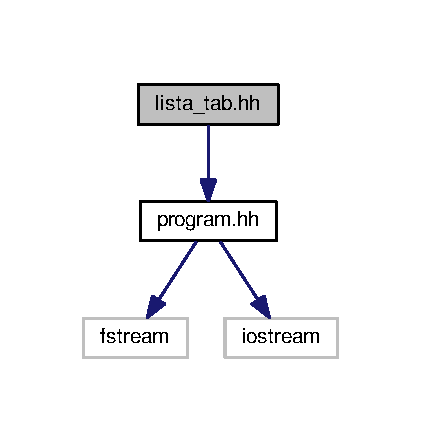
\includegraphics[width=202pt]{lista__tab_8hh__incl}
\end{center}
\end{figure}
Ten wykres pokazuje, które pliki bezpośrednio lub pośrednio załączają ten plik\-:
\nopagebreak
\begin{figure}[H]
\begin{center}
\leavevmode
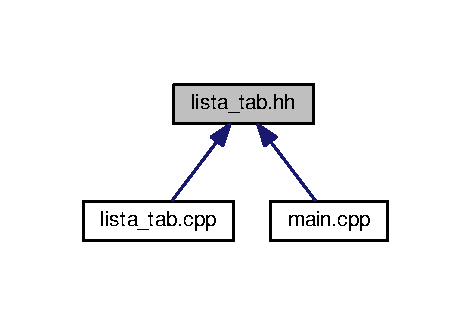
\includegraphics[width=226pt]{lista__tab_8hh__dep__incl}
\end{center}
\end{figure}
\subsection*{Komponenty}
\begin{DoxyCompactItemize}
\item 
class \hyperlink{class_lista__tab}{Lista\-\_\-tab}
\end{DoxyCompactItemize}
\subsection*{Definicje}
\begin{DoxyCompactItemize}
\item 
\#define \hyperlink{lista__tab_8hh_aa18bcf5b3ca1bcf8eb83ff54a925b132}{L\-I\-S\-T\-A\-\_\-\-\_\-\-T\-A\-B\-\_\-\-H\-H}
\end{DoxyCompactItemize}


\subsection{Dokumentacja definicji}
\hypertarget{lista__tab_8hh_aa18bcf5b3ca1bcf8eb83ff54a925b132}{\index{lista\-\_\-tab.\-hh@{lista\-\_\-tab.\-hh}!L\-I\-S\-T\-A\-\_\-\-\_\-\-T\-A\-B\-\_\-\-H\-H@{L\-I\-S\-T\-A\-\_\-\-\_\-\-T\-A\-B\-\_\-\-H\-H}}
\index{L\-I\-S\-T\-A\-\_\-\-\_\-\-T\-A\-B\-\_\-\-H\-H@{L\-I\-S\-T\-A\-\_\-\-\_\-\-T\-A\-B\-\_\-\-H\-H}!lista_tab.hh@{lista\-\_\-tab.\-hh}}
\subsubsection[{L\-I\-S\-T\-A\-\_\-\-\_\-\-T\-A\-B\-\_\-\-H\-H}]{\setlength{\rightskip}{0pt plus 5cm}\#define L\-I\-S\-T\-A\-\_\-\-\_\-\-T\-A\-B\-\_\-\-H\-H}}\label{lista__tab_8hh_aa18bcf5b3ca1bcf8eb83ff54a925b132}


Definicja w linii \hyperlink{lista__tab_8hh_source_l00003}{3} pliku \hyperlink{lista__tab_8hh_source}{lista\-\_\-tab.\-hh}.


\hypertarget{lista__tab_8hh}{\section{lista\-\_\-tab.\-hh}
\label{lista__tab_8hh}\index{lista\-\_\-tab.\-hh@{lista\-\_\-tab.\-hh}}
}

\begin{DoxyCode}
00001 \textcolor{comment}{//lista\_tab.hh}
00002 \textcolor{preprocessor}{#ifndef LISTA\_TAB\_HH}
\hypertarget{lista__tab_8hh_source_l00003}{}\hyperlink{lista__tab_8hh_aa18bcf5b3ca1bcf8eb83ff54a925b132}{00003} \textcolor{preprocessor}{}\textcolor{preprocessor}{#define LISTA\_\_TAB\_HH}
00004 \textcolor{preprocessor}{}
00005 \textcolor{preprocessor}{#include "\hyperlink{program_8hh}{program.hh}"}
00006 
\hypertarget{lista__tab_8hh_source_l00012}{}\hyperlink{class_lista__tab}{00012} \textcolor{keyword}{class }\hyperlink{class_lista__tab}{Lista\_tab}: \textcolor{keyword}{public} \hyperlink{class_program}{Program}\{
\hypertarget{lista__tab_8hh_source_l00016}{}\hyperlink{class_lista__tab_a59e0425d896070457d1f3456b91842fd}{00016}   \textcolor{keywordtype}{int} \hyperlink{class_lista__tab_a59e0425d896070457d1f3456b91842fd}{rozmiar};
\hypertarget{lista__tab_8hh_source_l00020}{}\hyperlink{class_lista__tab_afd2c6ba3ae15e658890641b188c7ed39}{00020}   \textcolor{keywordtype}{int} \hyperlink{class_lista__tab_afd2c6ba3ae15e658890641b188c7ed39}{iterator};
\hypertarget{lista__tab_8hh_source_l00024}{}\hyperlink{class_lista__tab_a123dfb670e5a5592e512c41cc4faf14e}{00024}   \textcolor{keywordtype}{int} *\hyperlink{class_lista__tab_a123dfb670e5a5592e512c41cc4faf14e}{tab};
00025 \textcolor{keyword}{public}:
\hypertarget{lista__tab_8hh_source_l00031}{}\hyperlink{class_lista__tab_af10d3131eadfebb4df8abbe6379e6d7c}{00031}  \hyperlink{class_lista__tab_af10d3131eadfebb4df8abbe6379e6d7c}{Lista\_tab}()\{
00032     \hyperlink{class_lista__tab_a123dfb670e5a5592e512c41cc4faf14e}{tab} = NULL;
00033     \hyperlink{class_lista__tab_a59e0425d896070457d1f3456b91842fd}{rozmiar} = 0;
00034     \hyperlink{class_lista__tab_afd2c6ba3ae15e658890641b188c7ed39}{iterator} = 0;
00035   \}
00036 
\hypertarget{lista__tab_8hh_source_l00043}{}\hyperlink{class_lista__tab_aaf55f952c14d2996c6f1e09acd718528}{00043}   \hyperlink{class_lista__tab_aaf55f952c14d2996c6f1e09acd718528}{~Lista\_tab}()\{\textcolor{keyword}{delete}[] \hyperlink{class_lista__tab_a123dfb670e5a5592e512c41cc4faf14e}{tab}; \hyperlink{class_lista__tab_a123dfb670e5a5592e512c41cc4faf14e}{tab}=NULL; \hyperlink{class_lista__tab_a59e0425d896070457d1f3456b91842fd}{rozmiar}=0; 
      \hyperlink{class_lista__tab_afd2c6ba3ae15e658890641b188c7ed39}{iterator}=0;\}
00044 
00052   \textcolor{keywordtype}{void} \hyperlink{class_lista__tab_a800998768639b41b5be5c52ec4ccbda4}{push}(\textcolor{keywordtype}{int} x);
00058   \textcolor{keywordtype}{void} \hyperlink{class_lista__tab_affc42a7ffc6eda21076fc56eae38e980}{pop}();
00066   \textcolor{keywordtype}{int} \hyperlink{class_lista__tab_af092dd7943f7cd5ff407485f2991a1e4}{size}();
00067 
00077   \textcolor{keywordtype}{bool} \hyperlink{class_program_ac396401ba5cade863d0e6acb727bec4e}{wykonaj\_program}(\textcolor{keywordtype}{char}* nazwa\_pliku,\textcolor{keywordtype}{int} ilosc\_danych);
00078 
00086   \textcolor{keywordtype}{void} \hyperlink{class_lista__tab_a506a6de79a600bac8316a6caf9878528}{wyczysc\_dane}(\textcolor{keywordtype}{int} ile);
00087 \};
00088 
00089 \textcolor{preprocessor}{#endif}
\end{DoxyCode}

\hypertarget{main_8cpp}{\section{Dokumentacja pliku main.\-cpp}
\label{main_8cpp}\index{main.\-cpp@{main.\-cpp}}
}
{\ttfamily \#include \char`\"{}A\-B\-Data/list.\-hh\char`\"{}}\\*
{\ttfamily \#include \char`\"{}A\-B\-Data/stack.\-hh\char`\"{}}\\*
{\ttfamily \#include \char`\"{}A\-B\-Data/queue.\-hh\char`\"{}}\\*
{\ttfamily \#include \char`\"{}A\-B\-Data/iterable.\-hh\char`\"{}}\\*
{\ttfamily \#include \char`\"{}Benchmark/timer.\-hh\char`\"{}}\\*
{\ttfamily \#include \char`\"{}Benchmark/benchmark.\-hh\char`\"{}}\\*
{\ttfamily \#include \char`\"{}Benchmark/observer.\-hh\char`\"{}}\\*
{\ttfamily \#include \char`\"{}Trees/binarytree.\-hh\char`\"{}}\\*
{\ttfamily \#include \char`\"{}A\-B\-Data/sorts.\-hh\char`\"{}}\\*
{\ttfamily \#include \char`\"{}A\-B\-Data/abdatatools.\-hh\char`\"{}}\\*
{\ttfamily \#include \char`\"{}A\-B\-Data/listarray.\-hh\char`\"{}}\\*
{\ttfamily \#include \char`\"{}assoctab.\-hh\char`\"{}}\\*
{\ttfamily \#include \char`\"{}Trees/redblacktree.\-hh\char`\"{}}\\*
{\ttfamily \#include \char`\"{}unistd.\-h\char`\"{}}\\*
Wykres zależności załączania dla main.\-cpp\-:
\nopagebreak
\begin{figure}[H]
\begin{center}
\leavevmode
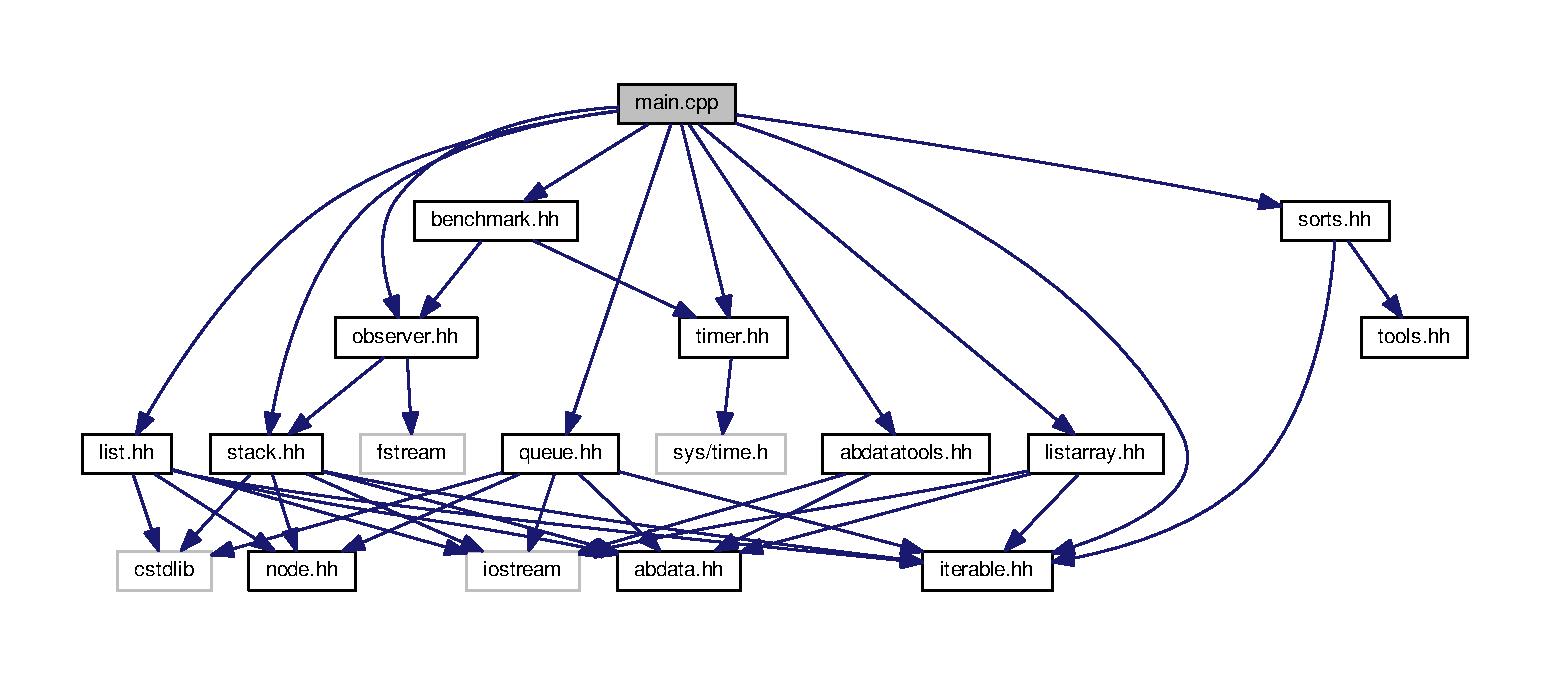
\includegraphics[width=350pt]{main_8cpp__incl}
\end{center}
\end{figure}
\subsection*{Funkcje}
\begin{DoxyCompactItemize}
\item 
int \hyperlink{main_8cpp_ae66f6b31b5ad750f1fe042a706a4e3d4}{main} ()
\end{DoxyCompactItemize}


\subsection{Dokumentacja funkcji}
\hypertarget{main_8cpp_ae66f6b31b5ad750f1fe042a706a4e3d4}{\index{main.\-cpp@{main.\-cpp}!main@{main}}
\index{main@{main}!main.cpp@{main.\-cpp}}
\subsubsection[{main}]{\setlength{\rightskip}{0pt plus 5cm}int main (
\begin{DoxyParamCaption}
{}
\end{DoxyParamCaption}
)}}\label{main_8cpp_ae66f6b31b5ad750f1fe042a706a4e3d4}


Definicja w linii \hyperlink{main_8cpp_source_l00018}{18} pliku \hyperlink{main_8cpp_source}{main.\-cpp}.



Oto graf wywołań dla tej funkcji\-:
\nopagebreak
\begin{figure}[H]
\begin{center}
\leavevmode
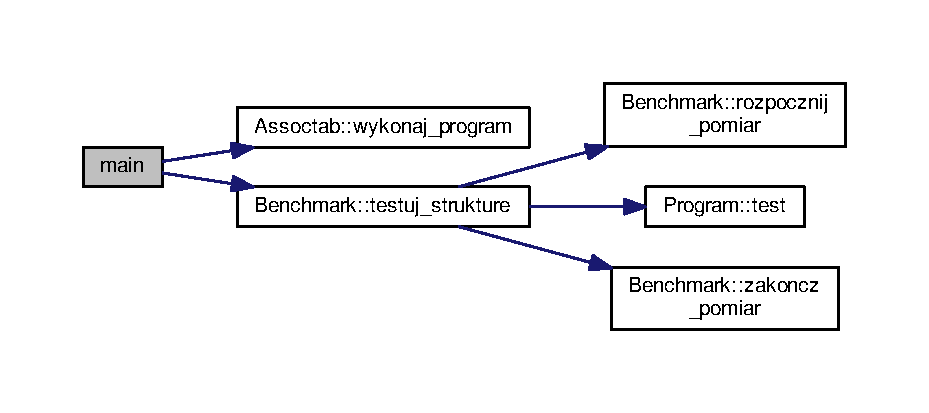
\includegraphics[width=350pt]{main_8cpp_ae66f6b31b5ad750f1fe042a706a4e3d4_cgraph}
\end{center}
\end{figure}



\hypertarget{main_8cpp}{\section{main.\-cpp}
\label{main_8cpp}\index{main.\-cpp@{main.\-cpp}}
}

\begin{DoxyCode}
00001 \textcolor{comment}{//main.cpp}
00002 \textcolor{preprocessor}{#include <iostream>}
00003 \textcolor{preprocessor}{#include "\hyperlink{program_8hh}{program.hh}"}
00004 \textcolor{preprocessor}{#include "\hyperlink{tabx2_8hh}{tabx2.hh}"}
00005 \textcolor{preprocessor}{#include "\hyperlink{benchmark_8hh}{benchmark.hh}"}
00006 \textcolor{preprocessor}{#include "\hyperlink{lista_8hh}{lista.hh}"}
00007 \textcolor{preprocessor}{#include "\hyperlink{lista__tab_8hh}{lista\_tab.hh}"}
00008 \textcolor{preprocessor}{#include "\hyperlink{assoctab_8hh}{assoctab.hh}"}
00009 
00010 \textcolor{keyword}{using namespace }std;
00011 
\hypertarget{main_8cpp_source_l00012}{}\hyperlink{main_8cpp_ae66f6b31b5ad750f1fe042a706a4e3d4}{00012} \textcolor{keywordtype}{int} \hyperlink{main_8cpp_ae66f6b31b5ad750f1fe042a706a4e3d4}{main}()\{
00013   \hyperlink{class_lista__tab}{Lista\_tab} a;
00014   \hyperlink{class_benchmark}{Benchmark} b;
00015   \textcolor{keywordtype}{char}* dane = (\textcolor{keywordtype}{char}*)\textcolor{stringliteral}{"dane.dat"};
00016   \textcolor{keywordtype}{int} ilosc\_testow = 10;
00017   
00018     a.\hyperlink{class_lista__tab_ac9adc6ecc7348c5e1871b239c1313405}{wykonaj\_program}(dane, 10);
00019     \textcolor{keywordflow}{for}(\textcolor{keywordtype}{int} i=0; i<=a.\hyperlink{class_lista__tab_afd2c6ba3ae15e658890641b188c7ed39}{iterator}; i++)
00020     cout<< a.\hyperlink{class_lista__tab_a123dfb670e5a5592e512c41cc4faf14e}{tab}[i]<<endl;
00021     a.\hyperlink{class_lista__tab_a409e9a4edbef4337980c7184b6cbfb63}{mergesort}(0,a.\hyperlink{class_lista__tab_afd2c6ba3ae15e658890641b188c7ed39}{iterator});
00022     cout<<endl<<endl;
00023     \textcolor{keywordflow}{for}(\textcolor{keywordtype}{int} i=0; i<=a.\hyperlink{class_lista__tab_afd2c6ba3ae15e658890641b188c7ed39}{iterator}; i++)
00024     cout<< a.\hyperlink{class_lista__tab_a123dfb670e5a5592e512c41cc4faf14e}{tab}[i]<<endl;
00025   
00026   \textcolor{comment}{/*}
00027 \textcolor{comment}{  for(int ilosc\_danych=1; ilosc\_danych<=10000000;ilosc\_danych*=10)\{}
00028 \textcolor{comment}{    cout << b.testuj\_strukture(a,dane,ilosc\_danych,ilosc\_testow) << endl;}
00029 \textcolor{comment}{  \}}
00030 \textcolor{comment}{  */}  
00031   \textcolor{keywordflow}{return} 0;
00032 \}
\end{DoxyCode}

\hypertarget{program_8cpp}{\section{Dokumentacja pliku program.\-cpp}
\label{program_8cpp}\index{program.\-cpp@{program.\-cpp}}
}
{\ttfamily \#include \char`\"{}program.\-hh\char`\"{}}\\*
{\ttfamily \#include $<$iostream$>$}\\*
{\ttfamily \#include $<$fstream$>$}\\*
{\ttfamily \#include $<$cstdlib$>$}\\*
Wykres zależności załączania dla program.\-cpp\-:
\nopagebreak
\begin{figure}[H]
\begin{center}
\leavevmode
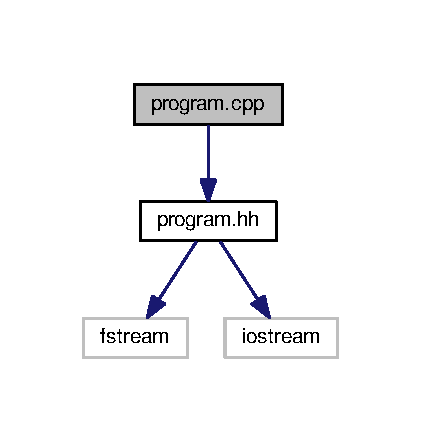
\includegraphics[width=318pt]{program_8cpp__incl}
\end{center}
\end{figure}

\hypertarget{program_8cpp}{\section{program.\-cpp}
\label{program_8cpp}\index{program.\-cpp@{program.\-cpp}}
}

\begin{DoxyCode}
00001 \textcolor{comment}{//program.cpp}
00002 \textcolor{preprocessor}{#include "\hyperlink{program_8hh}{program.hh}"}
00003 
00004 \textcolor{keyword}{using namespace }std;
\hypertarget{program_8cpp_source_l00008}{}\hyperlink{class_program_a618d9d6e3255ca5ff3d65de0385c6d46}{00008} \textcolor{keywordtype}{bool} \hyperlink{class_program_a618d9d6e3255ca5ff3d65de0385c6d46}{Program::wczytaj\_dane}(\textcolor{keywordtype}{char}* nazwa\_pliku)\{
00009   \textcolor{keywordflow}{if}(plik\_we.good()==\textcolor{keyword}{true})
00010     plik\_we.close();
00011   plik\_we.open(nazwa\_pliku);
00012   \textcolor{keywordflow}{if}(plik\_we.good()==\textcolor{keyword}{false})\{
00013     cerr<<\textcolor{stringliteral}{"Blad odczytu pliku!"};
00014     \textcolor{keywordflow}{return} \textcolor{keyword}{false};
00015   \}
00016   plik\_we >> rozmiar\_tab;
00017   tab=\textcolor{keyword}{new} \textcolor{keywordtype}{int} [rozmiar\_tab];
00018   \textcolor{keywordtype}{int} i=0;
00019   \textcolor{keywordflow}{while}(plik\_we >> tab[i])\{
00020     i++;
00021   \}
00022   plik\_we.close();
00023   \textcolor{keywordflow}{return} \textcolor{keyword}{true};
00024 \}
00025 
\hypertarget{program_8cpp_source_l00026}{}\hyperlink{class_program_a6bfc0c61a365d212dbb73e95034185c1}{00026} \textcolor{keywordtype}{bool} \hyperlink{class_program_a618d9d6e3255ca5ff3d65de0385c6d46}{Program::wczytaj\_dane}(\textcolor{keywordtype}{char}* nazwa\_pliku, \textcolor{keywordtype}{int} ile\_danych)\{
00027   \textcolor{keywordflow}{if}(plik\_we.good()==\textcolor{keyword}{true})
00028     plik\_we.close();
00029   plik\_we.open(nazwa\_pliku);
00030   \textcolor{keywordflow}{if}(plik\_we.good()==\textcolor{keyword}{false})\{
00031     cerr<<\textcolor{stringliteral}{"Blad odczytu pliku!"}<<endl;
00032     \textcolor{keywordflow}{return} \textcolor{keyword}{false};
00033   \}
00034   plik\_we >> rozmiar\_tab;
00035   \textcolor{keywordflow}{if}(ile\_danych>rozmiar\_tab)\{
00036     plik\_we.close();
00037     \textcolor{keywordflow}{return} \textcolor{keyword}{false};
00038   \}
00039   rozmiar\_tab=ile\_danych;
00040   tab=\textcolor{keyword}{new} \textcolor{keywordtype}{int} [ile\_danych];
00041   \textcolor{keywordflow}{for}(\textcolor{keywordtype}{int} i=0;i<ile\_danych;i++)
00042     plik\_we>>tab[i];
00043   plik\_we.close();
00044   \textcolor{keywordflow}{return} \textcolor{keyword}{true};
00045 \}
00046 
\hypertarget{program_8cpp_source_l00047}{}\hyperlink{class_program_a0a0d555a69e791820a70000375462e32}{00047} \textcolor{keywordtype}{bool} \hyperlink{class_program_a0a0d555a69e791820a70000375462e32}{Program::zapisz\_dane}(\textcolor{keywordtype}{char}* nazwa\_pliku)\{
00048   \textcolor{keywordflow}{if}(plik\_wy.good()==\textcolor{keyword}{true})
00049     plik\_wy.close();
00050   plik\_wy.open(nazwa\_pliku);
00051   \textcolor{keywordflow}{if}(plik\_wy.good()==\textcolor{keyword}{false})\{
00052     cerr<<\textcolor{stringliteral}{"Blad odczytu pliku!"};
00053     \textcolor{keywordflow}{return} \textcolor{keyword}{false};
00054   \}
00055   plik\_wy << rozmiar\_tab << endl;
00056   \textcolor{keywordflow}{for}(\textcolor{keywordtype}{int} i=0;i<rozmiar\_tab;i++)
00057     plik\_wy << tab[i] << endl;
00058   plik\_wy.close();
00059   \textcolor{keywordflow}{return} \textcolor{keyword}{true};
00060 \}
00061 
\hypertarget{program_8cpp_source_l00062}{}\hyperlink{class_program_ac939bc41859b867dd631163f6540573f}{00062} \textcolor{keywordtype}{void} \hyperlink{class_program_ac939bc41859b867dd631163f6540573f}{Program::wyswietl\_dane}()\{
00063   \textcolor{keywordflow}{for}(\textcolor{keywordtype}{int} i=0;i<rozmiar\_tab;i++)
00064     cout<<tab[i]<<endl;
00065 \}
00066 
\hypertarget{program_8cpp_source_l00067}{}\hyperlink{class_program_ac396401ba5cade863d0e6acb727bec4e}{00067} \textcolor{keywordtype}{bool} \hyperlink{class_program_ac396401ba5cade863d0e6acb727bec4e}{Program::wykonaj\_program}()\{
00068   cerr<<\textcolor{stringliteral}{"Nie wybrano programu do wykonania!"}<<endl;
00069   \textcolor{keywordflow}{return} \textcolor{keyword}{false};
00070 \}
\end{DoxyCode}

\hypertarget{program_8hh}{\section{Dokumentacja pliku program.\-hh}
\label{program_8hh}\index{program.\-hh@{program.\-hh}}
}


Definicja klasy \hyperlink{class_program}{Program}.  


{\ttfamily \#include $<$fstream$>$}\\*
{\ttfamily \#include $<$iostream$>$}\\*
Wykres zależności załączania dla program.\-hh\-:\nopagebreak
\begin{figure}[H]
\begin{center}
\leavevmode
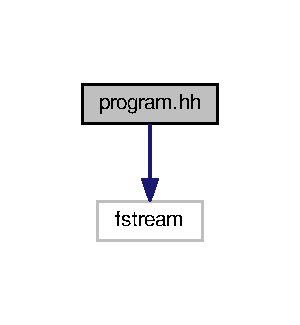
\includegraphics[width=202pt]{program_8hh__incl}
\end{center}
\end{figure}
Ten wykres pokazuje, które pliki bezpośrednio lub pośrednio załączają ten plik\-:
\nopagebreak
\begin{figure}[H]
\begin{center}
\leavevmode
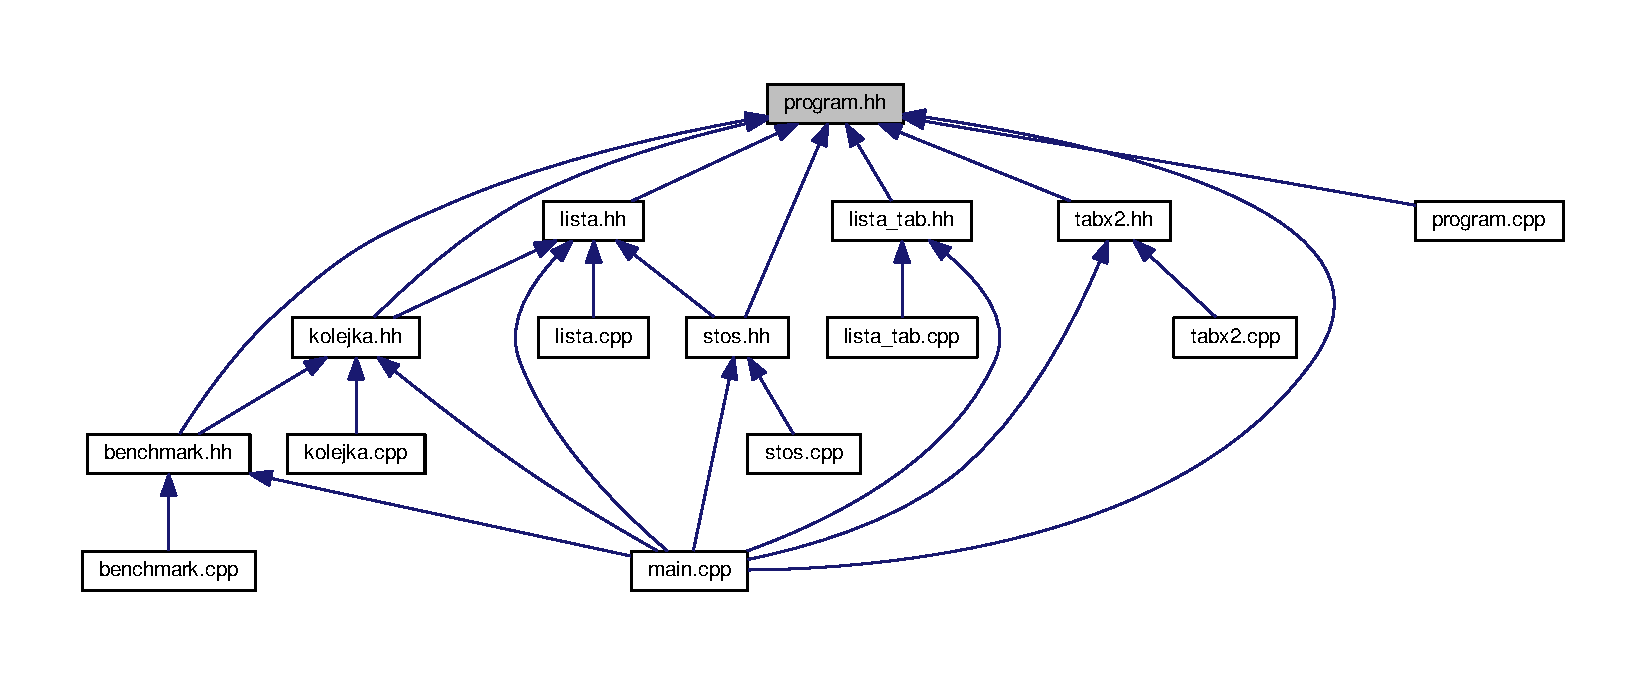
\includegraphics[width=350pt]{program_8hh__dep__incl}
\end{center}
\end{figure}
\subsection*{Komponenty}
\begin{DoxyCompactItemize}
\item 
class \hyperlink{class_program}{Program}
\begin{DoxyCompactList}\small\item\em Modeluje klase \hyperlink{class_program}{Program}. \end{DoxyCompactList}\end{DoxyCompactItemize}

\hypertarget{program_8hh}{\section{program.\-hh}
\label{program_8hh}\index{program.\-hh@{program.\-hh}}
}

\begin{DoxyCode}
00001 \textcolor{comment}{//program.hh}
00002 
00003 \textcolor{preprocessor}{#ifndef PROGRAM\_HH}
00004 \textcolor{preprocessor}{}\textcolor{preprocessor}{#define PROGRAM\_HH}
00005 \textcolor{preprocessor}{}
00006 \textcolor{preprocessor}{#include <fstream>}
00007 \textcolor{preprocessor}{#include <iostream>}
00008 
00009 \textcolor{keyword}{using namespace }std;
00010 
\hypertarget{program_8hh_source_l00022}{}\hyperlink{class_program}{00022} \textcolor{keyword}{class }\hyperlink{class_program}{Program}\{
00023 \textcolor{keyword}{protected}:
\hypertarget{program_8hh_source_l00031}{}\hyperlink{class_program_a3b5a10104019b9daa23ce4a5f5533820}{00031}   \textcolor{keywordtype}{int} \hyperlink{class_program_a3b5a10104019b9daa23ce4a5f5533820}{rozmiar\_tab};
00032 
\hypertarget{program_8hh_source_l00039}{}\hyperlink{class_program_ac72268c925315098b1632cc97d0f818a}{00039}   \textcolor{keywordtype}{int} *\hyperlink{class_program_ac72268c925315098b1632cc97d0f818a}{tab};
00040 
\hypertarget{program_8hh_source_l00047}{}\hyperlink{class_program_aac2f72538e24e533c327fe5546a59210}{00047}   ifstream \hyperlink{class_program_aac2f72538e24e533c327fe5546a59210}{plik\_we};
00048 
\hypertarget{program_8hh_source_l00055}{}\hyperlink{class_program_a59c1761a5ea875b3d5a4678928f3a1de}{00055}   ofstream \hyperlink{class_program_a59c1761a5ea875b3d5a4678928f3a1de}{plik\_wy};
00056 
00057 \textcolor{keyword}{public}:
\hypertarget{program_8hh_source_l00063}{}\hyperlink{class_program_a4fb9c2979a0dca1e14c75f4cc461bebd}{00063}   \textcolor{keywordtype}{int} \hyperlink{class_program_a4fb9c2979a0dca1e14c75f4cc461bebd}{getRozmiar\_tab}()\{\textcolor{keywordflow}{return} rozmiar\_tab;\}
00064 
\hypertarget{program_8hh_source_l00071}{}\hyperlink{class_program_aaefaa0df08f3484476fc4d61e97acbdc}{00071}   \hyperlink{class_program_aaefaa0df08f3484476fc4d61e97acbdc}{Program}()\{rozmiar\_tab=0;tab=NULL;\}
00072 
\hypertarget{program_8hh_source_l00079}{}\hyperlink{class_program_a986aef1c50e1d338a3315a47ba6df549}{00079}   \hyperlink{class_program_a986aef1c50e1d338a3315a47ba6df549}{~Program}()\{\textcolor{keyword}{delete}[] tab; tab=NULL;\}
00080 
00096   \textcolor{keywordtype}{bool} wczytaj\_dane(\textcolor{keywordtype}{char}* nazwa\_pliku);
00097 
00114   \textcolor{keywordtype}{bool} wczytaj\_dane(\textcolor{keywordtype}{char}* nazwa\_pliku, \textcolor{keywordtype}{int} ile\_danych);
00115 
00131  \textcolor{keywordtype}{bool} zapisz\_dane(\textcolor{keywordtype}{char}* nazwa\_pliku);
00132 
00138   \textcolor{keywordtype}{void} wyswietl\_dane();
00139 
00145   \textcolor{keyword}{virtual} \textcolor{keywordtype}{bool} wykonaj\_program();
00146 
00147   \textcolor{keyword}{virtual} \textcolor{keywordtype}{bool} wykonaj\_program(\textcolor{keywordtype}{char}* nazwa\_pliku, \textcolor{keywordtype}{int} ilosc\_danych)=0;
00148   \textcolor{keyword}{virtual} \textcolor{keywordtype}{void} wyczysc\_dane(\textcolor{keywordtype}{int} ile)=0;
00149 
\hypertarget{program_8hh_source_l00150}{}\hyperlink{class_program_ae866e995ea153f83031107c194f604e5}{00150}   \textcolor{keyword}{virtual} \textcolor{keywordtype}{void} \hyperlink{class_program_ae866e995ea153f83031107c194f604e5}{test}()\{\};
00151 \};
00152 
00153 \textcolor{preprocessor}{#endif}
\end{DoxyCode}

\hypertarget{tabx2_8cpp}{\section{Dokumentacja pliku tabx2.\-cpp}
\label{tabx2_8cpp}\index{tabx2.\-cpp@{tabx2.\-cpp}}
}


Plik zawiera metody klasy \hyperlink{class_tabx2}{Tabx2}.  


{\ttfamily \#include \char`\"{}tabx2.\-hh\char`\"{}}\\*
Wykres zależności załączania dla tabx2.\-cpp\-:
\nopagebreak
\begin{figure}[H]
\begin{center}
\leavevmode
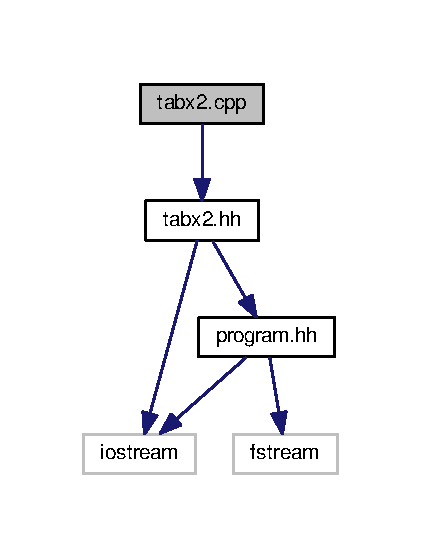
\includegraphics[width=202pt]{tabx2_8cpp__incl}
\end{center}
\end{figure}

\hypertarget{tabx2_8cpp}{\section{tabx2.\-cpp}
\label{tabx2_8cpp}\index{tabx2.\-cpp@{tabx2.\-cpp}}
}

\begin{DoxyCode}
00001 \textcolor{preprocessor}{#include "\hyperlink{tabx2_8hh}{tabx2.hh}"}
00002 
00003 \textcolor{keyword}{using namespace }std;
\hypertarget{tabx2_8cpp_source_l00007}{}\hyperlink{class_tabx2_a30db6636cba36a354443ec5f101fd188}{00007} \textcolor{keywordtype}{bool} \hyperlink{class_tabx2_a30db6636cba36a354443ec5f101fd188}{Tabx2::wykonaj\_program}()\{
00008   \textcolor{keywordflow}{if}(rozmiar\_tab==0)\{
00009     cerr<<\textcolor{stringliteral}{"Brak danych wejsciowych!"}<<endl;
00010     \textcolor{keywordflow}{return} \textcolor{keyword}{false};
00011   \}
00012   \textcolor{keywordflow}{for}(\textcolor{keywordtype}{int} i=0;i<rozmiar\_tab;i++)\{
00013     tab[i]*=2;
00014   \}
00015   \textcolor{keywordflow}{return} \textcolor{keyword}{true};
00016 \}
\end{DoxyCode}

\hypertarget{tabx2_8hh}{\section{Dokumentacja pliku tabx2.\-hh}
\label{tabx2_8hh}\index{tabx2.\-hh@{tabx2.\-hh}}
}


Definicja klasy \hyperlink{class_tabx2}{Tabx2}.  


{\ttfamily \#include $<$iostream$>$}\\*
{\ttfamily \#include \char`\"{}program.\-hh\char`\"{}}\\*
Wykres zależności załączania dla tabx2.\-hh\-:
\nopagebreak
\begin{figure}[H]
\begin{center}
\leavevmode
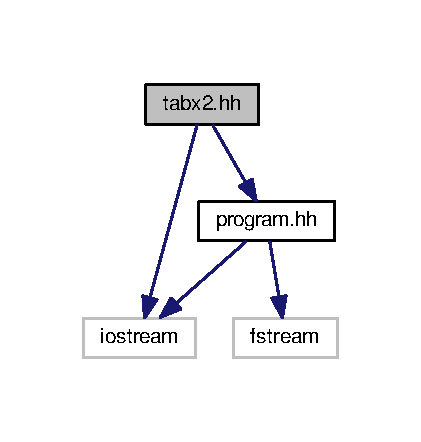
\includegraphics[width=217pt]{tabx2_8hh__incl}
\end{center}
\end{figure}
Ten wykres pokazuje, które pliki bezpośrednio lub pośrednio załączają ten plik\-:
\nopagebreak
\begin{figure}[H]
\begin{center}
\leavevmode
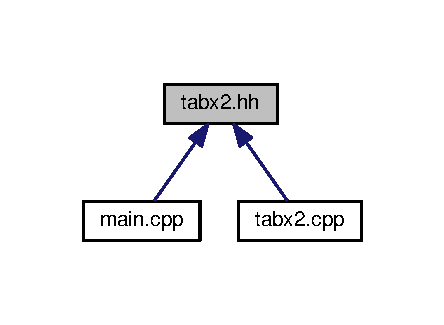
\includegraphics[width=213pt]{tabx2_8hh__dep__incl}
\end{center}
\end{figure}
\subsection*{Komponenty}
\begin{DoxyCompactItemize}
\item 
class \hyperlink{class_tabx2}{Tabx2}
\end{DoxyCompactItemize}


\subsection{Opis szczegółowy}
Klasa \hyperlink{class_tabx2}{Tabx2} jest klasa pochodna od klasy \hyperlink{class_program}{Program}. Definiuje metode podawajajaca kazda liczbe znajdujaca sie w tablicy danych wskazywanej przez zmienna tab klasy \hyperlink{class_program}{Program}. 

Definicja w pliku \hyperlink{tabx2_8hh_source}{tabx2.\-hh}.


\hypertarget{tabx2_8hh}{\section{tabx2.\-hh}
\label{tabx2_8hh}\index{tabx2.\-hh@{tabx2.\-hh}}
}

\begin{DoxyCode}
00001 \textcolor{comment}{//mnozenie\_tablicy.hh}
00002 
00003 \textcolor{preprocessor}{#ifndef TABX2\_HH}
00004 \textcolor{preprocessor}{}\textcolor{preprocessor}{#define TABX2\_HH}
00005 \textcolor{preprocessor}{}
00015 \textcolor{preprocessor}{#include <iostream>}
00016 \textcolor{preprocessor}{#include "\hyperlink{program_8hh}{program.hh}"}
00017 
\hypertarget{tabx2_8hh_source_l00018}{}\hyperlink{class_tabx2}{00018} \textcolor{keyword}{class }\hyperlink{class_tabx2}{Tabx2}: \textcolor{keyword}{public} \hyperlink{class_program}{Program}\{
00019 
00020 \textcolor{keyword}{public}:
00030   \textcolor{keyword}{virtual} \textcolor{keywordtype}{bool} \hyperlink{class_tabx2_a30db6636cba36a354443ec5f101fd188}{wykonaj\_program}();
00031 \};
00032 
00033 \textcolor{preprocessor}{#endif}
\end{DoxyCode}

\input{tmp_8hh}
\input{tmp_8hh_source}
%--- End generated contents ---

% Index
\newpage
\phantomsection
\addcontentsline{toc}{chapter}{Indeks}
\printindex

\end{document}
